\documentclass[listof=totocnumbered,bibliography=totocnumbered,12pt,oneside]{scrreprt}
\def\@afterindentfalse{\let\if@afterindent\iffalse}
\usepackage[english,german,ngerman]{babel}
\usepackage{geometry}
\usepackage{xltxtra}
\usepackage{lmodern}
\usepackage{textcomp}
\usepackage{graphicx}
\usepackage{chngcntr}
\usepackage{amsmath,amsfonts}
\usepackage{fancyvrb}
\usepackage{minted}
\usepackage{color}
\usepackage{url}
\usepackage{setspace}
\usepackage[noindentafter]{titlesec}
\usepackage{titletoc}
\usepackage{fancyhdr}
\usepackage{lastpage}
\usepackage{subfig}

\newfontfamily\headingfont[]{Avenir Heavy}
\definecolor{codebg}{rgb}{0.8,0.8,0.9}
\newminted{c++}{linenos=true,bgcolor=codebg,tabsize=4,showspaces=false}
\setcounter{secnumdepth}{3}
\setcounter{tocdepth}{3}
\counterwithout{footnote}{chapter}
\numberwithin{equation}{subsection}
\renewcommand\theequation{\arabic{equation}}
\setmainfont[Mapping=tex-text]{Avenir Book}
\setsansfont{Avenir Book}
\titleformat{\tableofcontents}{\Large\bfseries}{\headingfont}{0em}{}
\titleformat{\chapter}{\Large\bfseries}{\headingfont}{0em}{\thechapter\hspace{1em}}
\titleformat{\section}{\large\mdseries}{\headingfont}{0em}{\thesection\hspace{1em}}
\titleformat{\subsection}{\normalsize\mdseries}{\headingfont}{0em}{\thesubsection\hspace{1em}}
\titlespacing{\paragraph}{0pt}{3.5ex plus 1ex minus .2ex}{0pt}
\linespread{1.3}

\lhead[O,E]{}
\rhead[O,E]{Door Tracked AR}
\lfoot[O,E]{Seite \thepage\ von \pageref{LastPage}}
\cfoot[O,E]{}
\rfoot[O,E]{Kron, Ilic}
\renewcommand{\headrulewidth}{0.4pt}
\renewcommand{\footrulewidth}{0.4pt}

\fancypagestyle{plain}{
	\lhead[O,E]{}
	\rhead[O,E]{Door Tracked AR}
	\cfoot[O,E]{}
	\rfoot[O,E]{Kron, Ilic}
}

\makeatletter
\setlength{\@fptop}{0pt}
\makeatother

\begin{document}
\pagestyle{fancy}

\subject{Bachelor-Thesis}
\title{Door Tracked Augmented Reality}
\author{Mato Ilic \and David Kron}
\date{Januar 2014}
\publishers{Betreuer: Marcus Hudritsch\\Experte: Andreas Dürsteler}

\maketitle

\tableofcontents
\newpage

\chapter{Abstract}
Thema dieser Arbeit war, eine Augmented Reality Anwendung zu erstellen, welche Türen erkennt und Objekte (z.B. ein Vordach) über dieser Projeziert. Die Projektion soll dabei perspektivisch korrekt sein. Sprich, steht der Anwender seitlich zur Tür, dann sieh er auch das Vordach von der Seite. Die Anwendung sollte möglichst Plattformunabhängig sein. Aus diesem Grund sollten möglichst alle verwendeten Bibliotheken Teil des Projektes sein und spezifisch für dieses kompiliert werden. So soll die Installation erleichtert werden. Zur Umsetzung wurde die OpenCV Bibliothek verwendet, welche eine plattformübergreifendes Toolset für die Bildverarbeitung bietet. Die Darstellung der Ausgabe geschieht mittels OpenGL.
\newpage

\chapter{Einleitung}

Augmented Reality oder kurz AR ist eine computergestützte Erweiterung der Realitätswahrnehmung. Im Vergleich zur Virtual Reality, wo der Anwender in eine komplett künstlich generierte Welt eintaucht, geht es bei AR primär darum zusätzliche Informationen anzuzeigen, welche sich bestmöglich in die Umgebung einpassen. AR kann alle menschlichen Sinne erweitern, jedoch beschränkt sich die heutige Technologie primär darauf Live-Bilder oder Videos mit Zusatzinformationen mittels Einblendung oder Überlagerung zu ergänzen.

\section{Anwendungsgebiete}

Augmented Reality kann in allen Bereichen des Alltags eingesetzt werden. Bei der Navigation im Auto oder im Gebäude können Routen und Hinweise direkt in die Umgebung integriert werden, so dass der Benutzer nie das Auge von der Strasse abwenden muss. Ärzten kann AR dabei helfen gezielter zu arbeiten indem Röntgenaufnahmen während der Operation direkt auf den Patienten projiziert werden. Die Grundlagen hierfür sind meist die Gleichen wie in diesem Projekt. Objekterkennung, Positionsbestimmung und die Integration der Zusatzinformationen in die Umgebung.

\subsection{Medizin}

\begin{figure}[!ht]
\centering
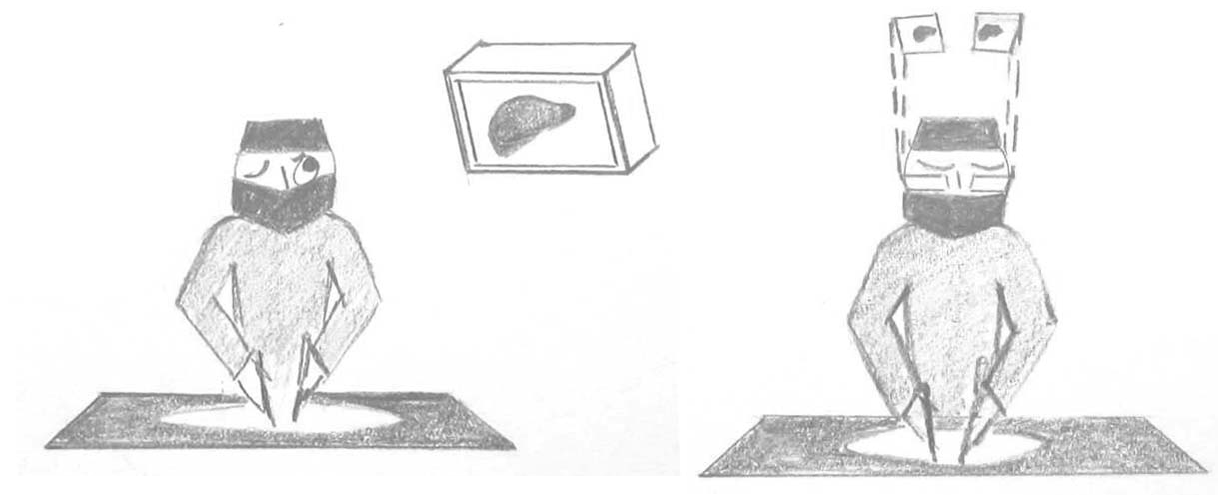
\includegraphics[scale=0.3]{images/vorteile_augmented_reality_medizin} 
\caption{Quelle: Suthau Tim, Berlin 2006, entnommen aus: Positionsgenaue Einblendung räumlicher Informationen in einem See Through Head Mounted Display für die Medizin am Beispiel der Leberchirurgie [Seite 13]}
\label{fig:ar-medicine}
\end{figure}

In der Medizin sind die Anwendungsmöglichkeiten von Augmented Reality vielfältig. Von der OP-Planung über die visuelle Navigation während der OP bis hin zur Telemedizin. Unterlagen wie Checklisten können zur Planung direkt Objektbezogen eingeblendet werden. So kann immer verfolgt werden wie die Vorbereitung des Patienten voranschreitet. Bei der Einrichtung des Operationssaals kann mittels AR direkt angezeigt werden, wo alles stehen muss um einen reibungslosen Ablauf der Operation zu garantieren. Während der Operation kann sich der Arzt voll und ganz auf den Patienten konzentrieren. Anstatt dass er seinen Blick immer wieder abwenden muss um z.B. Röntgenaufnahmen zu betrachten, werden diese direkt in das Sichtfeld projiziert. Speziell bei minimalinvasiven Eingriffen können so auch direkt die Navigationswege dargestellt werden, was die Präzision des Eingriffes erhöht.
\paragraph{}
Im Bereich der Telemedizin können Spezialisten dem ausführenden Arzt Hilfestellungen während der Diagnose oder Operation einblenden. Mediziner können so weltweit in Echtzeit kooperieren.

\subsection{Marketing}

\begin{figure}[!ht]
\centering
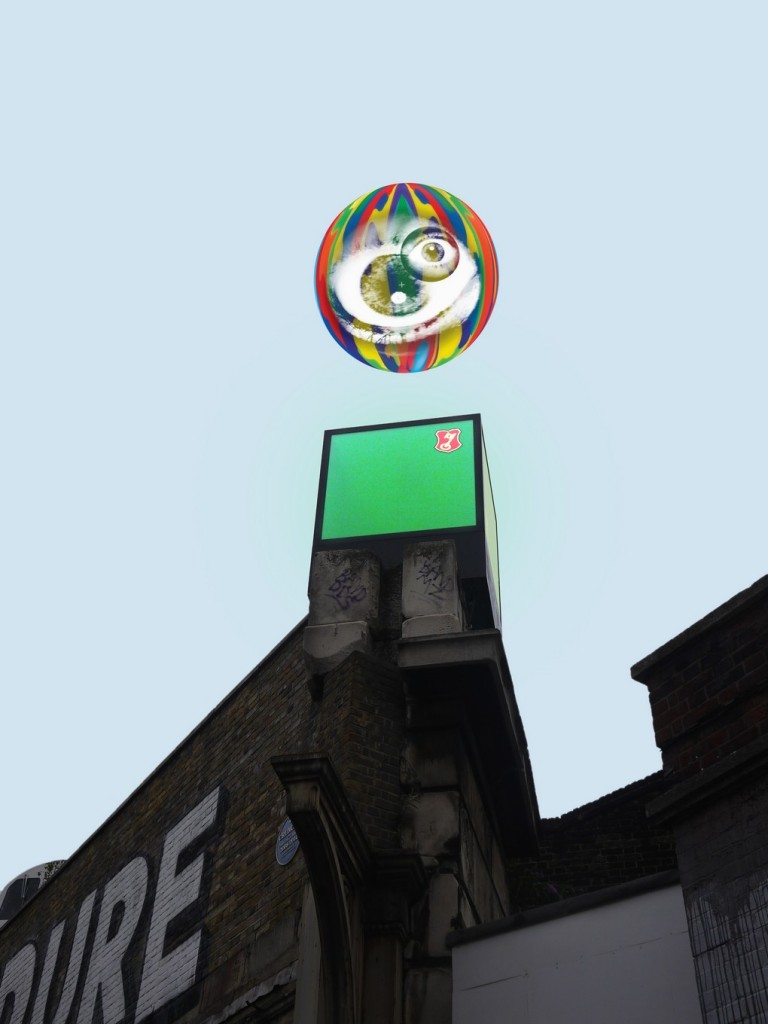
\includegraphics[scale=0.3]{images/ar-marketing} 
\caption{Becks Green Box Kampagne. Quelle: http://www.i-ref.de/2011/12/06/beck's-green-box-projekt-augmented-reality-in-berlin}
\label{fig:ar-marketing}
\end{figure}

Auch im Bereich des Marketing bietet Augented Reality unzählige neue Möglichkeiten. Tablets und Smartphones sind fester Bestandteil des Alltags geworden. Bietet man den Kunden die Möglichkeit Produkte und Brands interaktiv in ihrer Umgebung zu entdecken, so hinterlässt dies einen bleibenden Eindruck und erhöht die Bindung zur Marke. Ein Vorreiter war hier die Firma Becks im vergangenen Jahr. Um den Kunden das Produkt näher zu bringen hat Becks in Grossstädten weltweit grüne Boxen aufgestellt. Haben die Benutzer ihr Smartphone dann auf diese gerichtet, bot sich ihnen eine bunte 3D-Show. Direkt in ihrer gewohnten Umgebung im Herzen der Städte. Nach dieser Kampagne konnte Becks einen signifikaten Anstieg des Absatzes in der betroffenen Städten feststellen und gewann weltweit neue Fans.

\paragraph{}
Dies sind nur zwei mögliche Anwendungsgebiete. Bereits wird AR auch in der Automobilbranche in Form von Overhead Displays eingesetzt. Im Militärbereich wird AR für die Einsatzkoordination in Kriegsgebieten verwendet.

\section{Aktuelle Entwicklungen}

\begin{figure}[!ht]
\centering

\includegraphics[width=\textwidth]{images/google-glass} 
\caption{Google Glass. Quelle: http://www.google.com/glass/start}
\label{fig:google-glass}
\end{figure}
\noindent
Bisher wurde das volle Potentiel von Augmented Reality nicht ausgeschöpft. Viele Anwendungen basieren immer noch auf sogenannten Markern, ähnlich wie QR-Codes, welche benötigt werden um zu bestimmen was und wo dargestellt werden muss. Die zweite Generation von AR-Applikationen ist jedoch auf dem Vormarsch. Diese können dank GPS und diverser anderer Sensoren in den Smartdevices auf Marker verzichten. Die Katalog-App von IKEA\footnote{\protect\url{http://mashable.com/2012/07/19/ikea-augmented-reality-catalog/}} und die TV Buying Guide App von Philips\footnote{\protect\url{http://www.youtube.com/watch?v=YBU0f0apgM0}} bauen beide auf diesen neuen Möglichkeiten auf. Augmented Reality Anwendungen haben im Jahr 2013 weltweit schätzungweise einen Umsatz von \$300 Millionen generiert\footnote{\protect\url{Quelle: http://www.juniperresearch.com/viewpressrelease.php?pr=348}}.
\paragraph{}
Die zur Zeit fortschrittlichsten Anwendungen von AR sind im Bereich der tragbaren Devices zu finden, allen voran Google Glass\footnote{\protect\url{http://www.google.com/glass/start}}. Mit Glass integriert Google Smartphonefunktionalität in Brillen. Die Meta Glasses\footnote{\protect\url{https://www.spaceglasses.com/}} gehen noch einen Schritt weiter und integrieren eine Microsoft Kinect ähnliche Kamera, welche eine präzise Erkennung von Gesten erlauben soll. Dies soll eine Interaktion mit Augmented Reality Objekten erlauben. Das Produkt soll im Juli 2014 Marktreife erreichen. Apple und Microsoft haben diverse Patente eingereicht, welche darauf hindeuten, dass auch sie an entsprechendem Equipment arbeiten.
\newpage

\chapter{Grundlagen}

Die Positionsbestimmung besteht aus drei elementaren Teilen. Der Kamerakalibrierung, welche das Bild entzerrt und wichtige Parameter der Kamera zurückliefert, welche für die Bestimmung der Perspektive wichtig sind. Anhand dieser Daten wird mittels der von OpenCV bereitgestellten Funktion die Perspektive von der Kamera zur Projektionsfläche bestimmt. Zuletzt wird mit Hilfe von Rodrigues die Rotation der Projektionsfläche angepasst. Diese drei Teile wollen wir hier nun etwas detaillierter erklären.

\section{Kamerakalibrierung}
Unsere Motivation einen Kalibrierungsprozess in die Applikation einzubauen war zum einen um zu verifizieren, ob unsere eingesetzten Kameras, wie von uns angenommen, verzerrungsfrei arbeiten. Zum anderen benötigen wir die intrinsischen Parameter der Kamera um ein Objekt korrekt in eine Augmented Reality Szene projizieren zu können. Die extrinsischen Parameter sind in unserem Fall zweitrangig, da diese von der Position der Kamera zur Projektionsfläche abhängen und somit zur Laufzeit stetig neu berechnet werden müssen.
\paragraph{}
Die Kalibrierung an sich umfasst die Analyse einer Serie von Projektionen von charakteristischen Punkten eines Musters, wobei die Position dieser "Feature Points" mit hoher Präzision bekannt ist. Die Position und die Distanz zwischen den einzelnen Punkten innerhalb der Projektion liefern Rückschlüsse bezüglich der Verzerrung innerhalb von dieser als auch Informationen bezüglich der intrinsischen und extrinsischen Eigenschaften des Aufnahmegerätes. 
\paragraph{}
Das Muster welches in diesem Projekt verwendet wurde ist ein Schachbrett. Durch die hohen Kontraste eines Schachbrettes lassen sich die Schnittpunkte der einzelnen Kacheln mit einer sehr hohen Präzision ermitteln. Die Projektionen sind in unserem Fall Aufnahmen des Schachbrettes aus verschiedenen Blickrichtungen. Wir haben uns für diese Basis für den Kalibrierungsprozess entschieden, weil diese sich in diversen Projekten bewährt hat und weil OpenCV bereits entsprechende Funktionen enthält um mit dieser Datengrundlage die Kalibrierung zu vollziehen. 

\section{Intrinsische Parameter}
Die intrinsischen Parameter einer Kamera bestehen aus zwei Komponenten: der Brennweite $f_x$ und $f_y$ und der Abweichung des Zentrum des Sensors zur optischen Bildmitte $c_x$ und $c_y$. Was diese zwei Eigenschaften beschreiben ist die interne Geometrie der Kamera, d.h. wie die aufgenommene Szene in ein 2D-Bild abgebildet wird. Somit ist klar, warum diese Parameter für die Ermittlung der Perspektive so wichtig sind. Zu beachten ist, dass die ermittelte Brennweite $f$ nicht die physische Brennweite sondern eine Kombination $Fs$ ist. $F$ gibt die Brennweite in mm an und $s$ die Skalierung von Pixel pro mm auf dem Sensor. Somit kann mittels $f$ die Pixelinformation bestimmt werden. Das Resultat ist eine einfache Abbildung eines Weltpunktes $(X, Y, Z)$ auf einen Bildpunkt $(x_i, y_i)$ welche wie folgt beschrieben ist.

\begin{equation}
x_i = f_x (\frac{X}{Z}) + c_x,   y_i = f_y (\frac{Y}{Z}) + c_y
\end{equation}

Diese zwei Operationen können nun auch in eine homogene Operation zusammengefasst werden.

\begin{equation}
\begin{bmatrix}
x \\ y \\ w
\end{bmatrix} 
=
\begin{bmatrix}
f_x & 0 & c_x \\
0 & f_y & c_y \\
0 & 0 & 1
\end{bmatrix} 
\begin{bmatrix}
X \\ Y \\ Z
\end{bmatrix} 
\end{equation}

Da die intrinsischen Parametereigenschaften der Hardware und unabhängig von der Umgebung sind, müssen sie für jedes Aufnahmegerät nur einmal zu Begin bestimmt werden und können anschliessend fix in der Applikation hinterlegt werden.

\section{Verzerrung}
Es gibt zwei Arten von Verzerrungen welche bei Aufnahmen mit Kameras entstehen können: radiale und tangentiale. Radiale Verzerrungen sind auf die gewölbte Form der Linsen zurückzuführen. Im Zentrum des Bildes ist die radiale Verzerrung noch bei null und nimmt gegen den Rand immer wie stärker zu. Theoretisch währe es möglich eine nahezu perfekte parabolische Linse herzustellen, jedoch wäre diese viel zu kostspielig in der Produktion. Deshalb werden allgemein sphärische Linsen eingesetzt.

\begin{figure}[!ht]
\centering
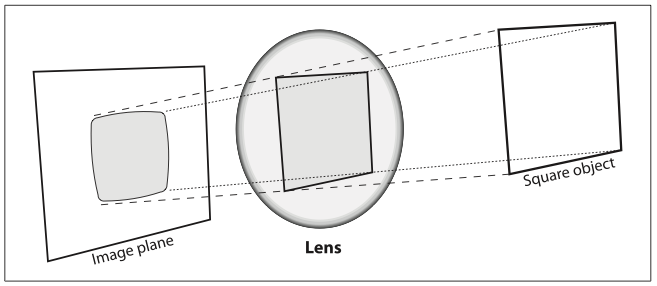
\includegraphics[scale=0.5]{images/radial-disortion.png} 
\caption{Strahlen welche die Linse weiter weg vom Zentrum passieren werden stärker abgelenkt als solche nahe dem Zentrum. Darum erschein die Projektion verzerrt.\protect\cite{learningopencv}}
\label{fig:radial-disortion}
\end{figure}

Tangentiale Verzerrungen werden durch Ungenauigkeiten bei der Zusammensetzung des optischen Systems verursacht. Diese entstehen, wenn die Linse nicht komplett parallel zum Sensor steht.

\begin{figure}[!ht]
\centering
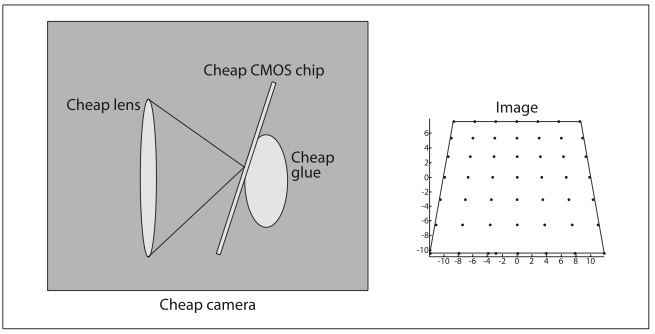
\includegraphics[scale=0.5]{images/tangential-disortion.png} 
\caption{Tangentiale Verzerrung aufgrund von Fehlern im optischen System.\protect\cite{learningopencv}}
\label{fig:tangential-disortion}
\end{figure}

\section{Koordinatensysteme}
Um den Kalibrierungsprozess zu verstehen, muss man auch die einzelnen Koordinatensysteme kennen, welche bei der Aufnahme eines Bildes durchlaufen werden. Deshalb möchten wir diese Hier kurz erläutern.

\paragraph{Weltkoordinatensystem} Dieses ist das Koordinatensystem in welchen die "reale Welt" gemessen wird und ist dreidimensional. Dies ist der Ursprung der Bilddaten.

\paragraph{Standardkoordinatensystem} Dieses dreidimensionale Koordinatensystem hat den Ursprung im Projektionszentrum. Seine Z-Achse verläuft entlang der optischen Achse.

\paragraph{Bildkoordinatensystem} Dieses hat seinen Ursprung beim Schnittpunkt der optischen Achse und der Bildebene. Die x- und y-Achse sind parallel zur X- bzw. Y-Achse des Standardkoordinatensystems.

\paragraph{Pixelkoordinatensystem} Das Pixelkoordinatensystem hat seinen Ursprung beim Korrigierten Punkt $c_x$ \/ $c_y$  und seine x- und y-Achse sind parallel zur x- bzw. y-Achse des Bildkoordinatensystem.

\paragraph{} Während dem Abbildungsprozess durchlaufen die einzelnen Bildimformationen nun diese Systeme wie folgt: Weltkoordinaten $\Rightarrow$ Standardkoordinaten $\Rightarrow$ Bildkoordinaten $\Rightarrow$ Pixelkoordinaten

\section{Implementierung}
Die Funktionalität für die Kalibrierung ist in der Klasse CameraCalibration implementiert. Da alle benötigten Algorithmen bereits in OpenCV implementiert sind, ist der Kalibrierungsprozess relativ einfach umzusetzen. OpenCV selbst verwendet das Verfahren, welches 1998 von Zhang\cite{zhang} entwickelt wurde. Dabei werden die einzelnen Parameter nicht exakt berechnet sondern mittels einer "Maximum likelihood estimation" mit einer hohen Präzision geschätzt. Eine präzise Schätzung erfordert jedoch eine breite Datenbasis. Deshalb reicht es nicht aus, nur eine Aufnahme des Schachbrettmusters als Input zu liefern. Empfohlen werden 15 - 20 Aufnahmen aus möglichst verschiedenen Blickwinkeln. Da die Erkennung des Musters nicht 100\% treffgenau ist, haben wir uns dazu entschieden immer min. 20 Aufnahmen zu verwenden. So können wir davon ausgehen, dass immer mehr als 15 erfolgreiche Erkennungen stattfinden.

\paragraph{}
Die Funktion \textit{CameraCalibration::cornerSubPix} akzeptiert eine Liste von aufnahmen des Schachbrettmusters. Als zweiter Parameter muss die Grösse des Brettes angegeben werden (die Anzahl innerer Eckpunkte in horizontaler und vertikaler Richtung). Dabei sollten die Breite ungerade und die Höhe gerade sein und das Muster sollte breiter als hoch sein. Wir haben uns für ein 6x9 grosses Muster entschieden, da dies die geläufigste Grösse zu sein scheint. Nun wird mittels \textit{CameraCalibration::findChessboardPoints} die Erkennung durchgeführt. Dabei müssen die \textit{objectCorners} (Bildkoordinatensystem) auf einen initialen Erwartungswert gesetzt werden.

\begin{c++code}
for(int i = 0; i < boardSize.height; i++)
{
    for(int j = 0; j < boardSize.width; j++)
    {
        //110 = size of one square on the board
        objectCorners.push_back(
            cv::Point3f(i * 110, j * 110, 0.0f)
        );
    }
}
\end{c++code}

Diese Punkte werden für die Erkennung des Schachbrettes noch nicht benötigt sondern erst bei der Kalibrierung. Anschliessend wird die OpenCV eigene Funktion zur Ermittlung des Musters aufgerufen.

\begin{c++code}
cv::findChessboardCorners(
    image, 
    boardSize, 
    imageCorners, 
    CV_CALIB_CB_ADAPTIVE_THRESH | CV_CALIB_CB_FILTER_QUADS
);
\end{c++code}

Da \textit{cv::findChessboardCorners} nur die ungefähre Position der Eckpunkte ermittelt, müssen die ermittelten Daten mit Hilfe von \textit{cv::cornerSubPix} verfeinert werden. Würde man dies nicht tun, so würde es zu Fehlern bei der Kalibrierung führen. Das genaue Vorgehen der Funktion kann der OpenCV Dokumentation \footnote{\protect\url{http://opencv.willowgarage.com/documentation/cpp/imgproc\_feature\_detection.html\#cv-cornersubpix}} entnommen werden.

\paragraph{}War die Erkennung des Schachbrettes erfolgreich, so entspricht die Anzahl an gefundenen \textit{imageCorners} der zuvor definierten Brettgrösse von 9x6, sprich 54. Alle erfolgreichen Versuche werden anschliessend in einer Liste abgelegt. Was zu beachten ist, und was uns einiges an Zeit gekostet hat, ist, dass die \textit{imageCorners} und die \textit{objectCorners} die gleiche Dimension haben müssen. Ist dies nicht der Fall, so schlägt die Kalibrierung mit einer kryptischen Meldung fehl.

\paragraph{} Nun kann mittels \textit{CameraCalibration::calibrate} die Kalibrierung vorgenommen werden. Diese ist die Voraussetzung für die anschliessende Entzerrung des Bildes welche in \textit{CameraCalibration::remap} stattfindet. Nach jeder Kalibrierung müssen die Daten für die Entzerrung initialisiert werden. Hier ist auch der Punkt, wo wir die Kameramatrix erhalten, welche die intrinsischen Parameter enthält.

\section{Auswertung} Das nun entzerrte Bild kann mit dem Ursprungsbild verglichen werden um zu eruieren ob das optische System Verzerrungen verursacht (Abb. \ref{fig:chessboard-disorted} und \ref{fig:chessboard-undisorted}). Bei den von uns getesteten Kameras konnten wir keine Verzerrungen feststellen. Dabei würden zwei Smartphone-Kameras (iPhone 4 und HTC Desire Z) und zwei Webcams (iSight Kamera eines MacBook Pro und die integrierte Kamera eines HP Notebooks) getestet. Hier stellt sich aber die Frage, ob die getesteten optischen Systeme so kompakt sind, dass die Verzerrungen optisch nicht erfasst werden können oder ob auf Hardwareebene bereits eine Korrektur stattfindet und die API nur Zugriff auf dieses Bild hat. Hierzu konnten wir Seitens der Hardwarehersteller keine Informationen finden.

\begin{figure}[!ht]
\centering
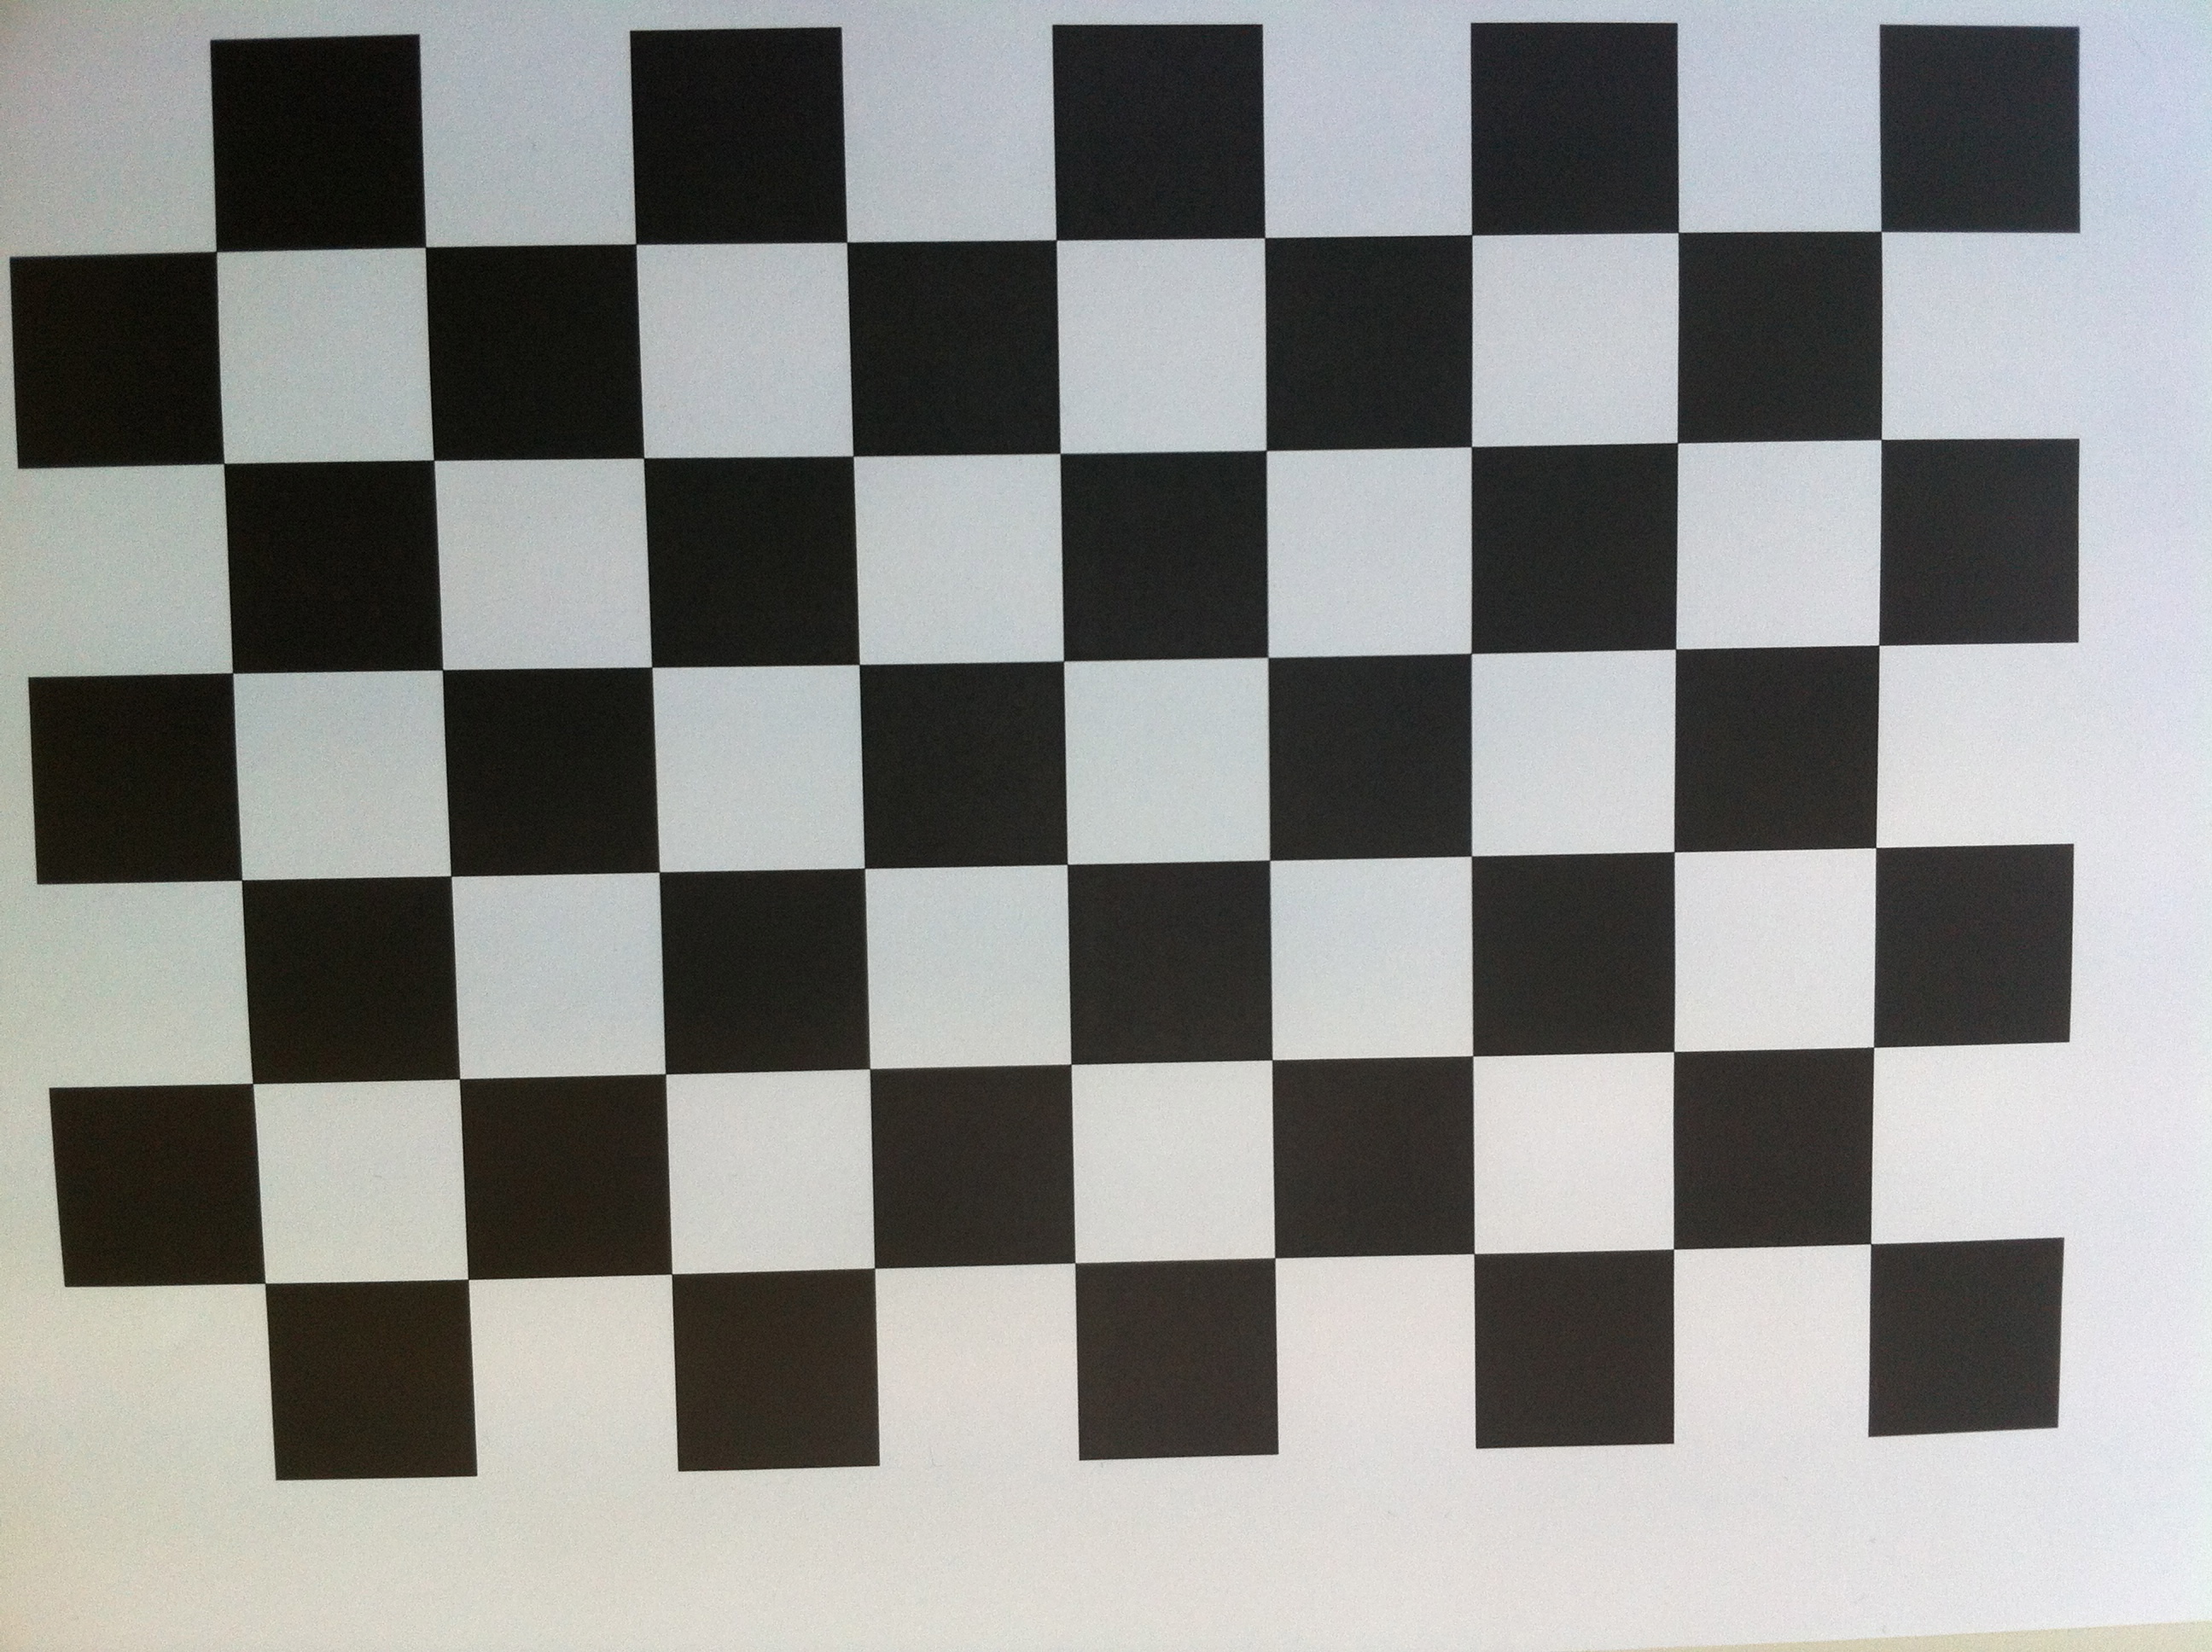
\includegraphics[scale=0.1]{images/chessboard-disorted.jpg} 
\caption{Originalbild}
\label{fig:chessboard-disorted}
\end{figure}

\begin{figure}[!ht]
\centering
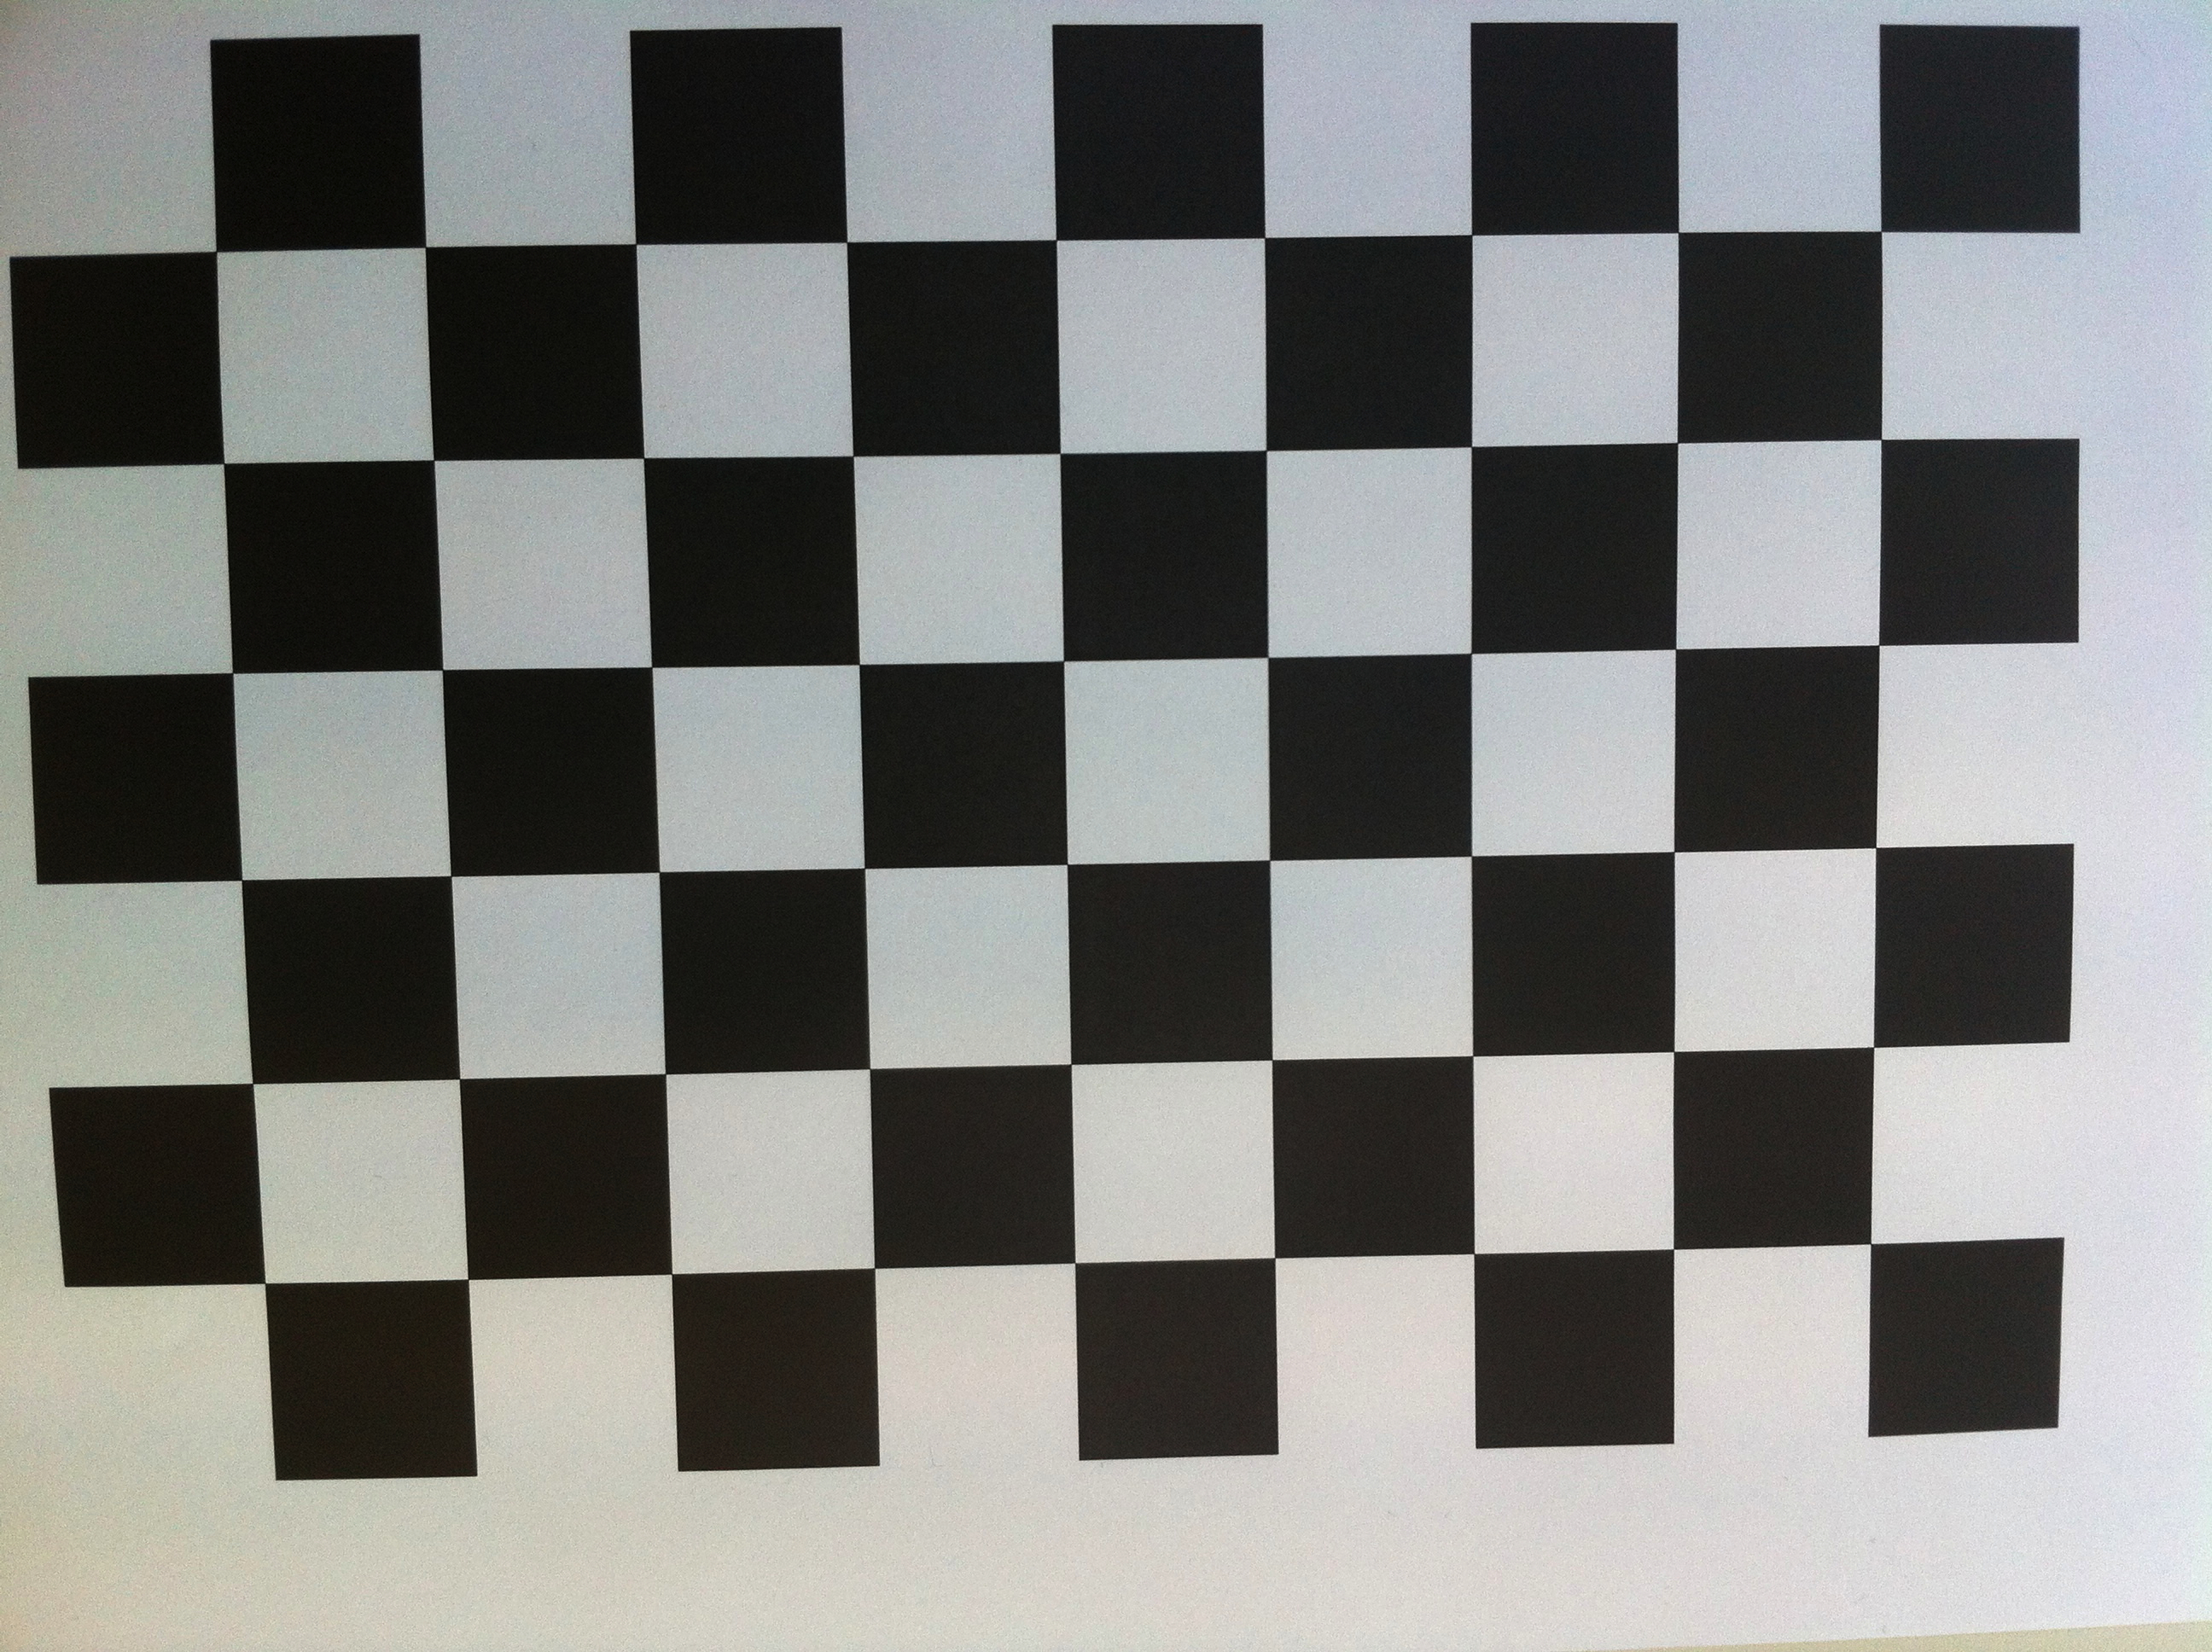
\includegraphics[scale=0.1]{images/chessboard-undisorted.jpg} 
\caption{Entzertes Bild}
\label{fig:chessboard-undisorted}
\end{figure}

\subsection{Perspektive}

\section{Projektionsmodell}
\label{sec:projektionsmodell}

Alle Funktionen in OpenCV arbeiten nach dem sogenannten Pinhole Camera Modell. Dabei werden die 3D-Punkte einer Szene mittels perspektivischer Transformation auf die Bildebene projiziert.

\begin{equation}
\vec{p^p} = K [R|t] \vec{p^i}
\end{equation}

Die ausgeschriebene Form zum besseren Verständnis:

\begin{equation}
\begin{bmatrix}	
p^c_x \\ p^c_y \\ 1
\end{bmatrix} 
=
\begin{bmatrix}
f_x & 0 & c_x \\
0 & f_y & c_y \\
0 & 0 & 1
\end{bmatrix} 
\begin{bmatrix}
r_{11} & r_{12} & r_{13} & t_1 \\
r_{21} & r_{22} & r_{23} & t_2 \\
r_{31} & r_{32} & r_{33} & t_3
\end{bmatrix} 
\begin{bmatrix}
p^i_x \\ p^i_y \\ p^i_z \\ 1
\end{bmatrix} 
\end{equation}

Ein Punkt $(p^i_x, p^i_y, p^i_z)$ im dreidimensionalen Raum wird dadurch auf einen zweidimensionalen Punkt in der Bildebene projiziert. Die Kamera-Matrix $K$ enthält dabei die intrinsischen Parameter und welche nur einmal zu Begin berechnet werden müssen. Die kombinierte Rotations- und Translationsmatrix $[R|t]$ überführt Objekt- in Kamera-Koordinaten, also in die Position, aus der das Objekt von der Kamera gesehen wird. Diese Matrix stellt die extrinsischen Parameter dar und muss anhand einer \textit{Pose Estimation} berechnet werden.

\section{Pose Estimation}
Bei der 3D Pose Estimation wird die Position sowie die Rotation eines Objekts in einem zweidimensionalen Bildes berechnet. Dadurch erhält man die Position des 3D-Objekts im dreidimensionalen Objektraum. Es gibt eine vielzahl an Algorithmen die sich diesem Problem widmen.

\paragraph{}
Zusätzliche Details zu diesem Thema folgen in Kapitel \ref{chap:projektion}.


\section{Rotation}
Eine 3x3 Matrix ist die geläufigste Methode wenn es darum geht eine Rotation im Raum zu vollziehen. Multipliziert man den Vektor mit der Matrix welche die entsprechenden Parameter enthält, so erhält man als Resultat den rotierten Vektor. Der Nachteil dabei ist, dass man für die Rotation jeder Achse andere Parameter der Matrix anpassen muss. Man kann die drei Matrizen zu einer zusammenfassen, jedoch wird die Prozedur dadurch noch unübersichtlicher. Da die Rotationsmatrizen nur drei Freiheitsgrade haben, ist der Gedanke nahe, die Informationen in einen Vektor abzubilden. Und genau hier setzt die in OpenCV implementierte Rodrigues-Transformation an. Nicht nur für uns Menschen ist ein Vektor einfacher lesbar, auch für numerische Optimierungen ist es einfacher mit einem Drei-Komponenten-Vektor zu arbeiten als mit einer 3x3 Matrix.

\paragraph{}
Rodrigues nutzt die Richtung des Vektors um die Rotationsachse und die Länge des Vektors um den Winkel der Rotation – im Gegenuhrzeigersinn – abzubilden. Sei $r$ ein dreidimensionaler Vektor 

\begin{equation}
\begin{pmatrix} r_x \\ r_y \\ r_z \end{pmatrix}
\end{equation}

Dieser Vektor bildet implizit den Winkel anhand seiner Länge ab.

\begin{equation}
\theta = \sqrt{{r_x}^2 + {r_y}^2 + {r_z}^2}
\end{equation}

Anhand dieser Repräsentation kann die Rotationsmatrix wie folgt wieder hergestellt werden:

\begin{equation}
R = \cos(\theta) * I + (1 - \cos(\theta)) * r * r^T + \sin(\theta) * 
\begin{bmatrix}
0 & -r_z & r_y \\
r_z & 0 & -r_x \\
r_y & r_x & 0
\end{bmatrix}
\end{equation}

Umgekehrt kann man aus der Rotationsmatrix die Rodrigues-Darstellung wie folgt ableiten:

\begin{equation}
\sin(\theta) * 
\begin{bmatrix}
0 & -r_z & r_y \\
r_z & 0 & -r_x \\
r_y & r_x & 0
\end{bmatrix}
= 
\frac{R - R^T}{2}
\end{equation}

Und genau diese zwei Möglichkeiten sind in \textit{cv::Rodrigues} implementiert. Wird als erster Parameter ein 3D-Vektor und als zweiter eine 3x3 Matrix übergeben so wird der Vektor zu einer Matrix transformiert. Will man die Operation umkehren, so müssen nur die Parameter-Typen in umgekehrter Reihenfolge übergeben werden.

\newpage

\chapter{Türerkennung}

Die Türerkennung erfolgt in mehreren Schritten. Zuerst wird im Bild nach Liniensegmenten gesucht. Die gefundenen Segmente müssen hinsichtlich Länge und Ausrichtung optimiert werden. Anschliessend muss nach möglichen Vier-Kanten-Paaren gesucht werden, welche möglicherweise eine Tür bilden. Die gefundenen Kandidaten werden dann noch evaluiert, um den besten Treffer zu bestimmen.

\section{Kantendetektion}

Es existieren verschiedene Algorithmen um Kanten in Bildern zu suchen. In dieser Arbeit wurden speziell die \textit{Probabilistic Hough Transform} und die \textit{Line Segment detection using Weighted Mean-Shift} oder kurz LSWMS untersucht. Beide sind darauf spezialisiert Geraden zu finden, wobei es merkliche Unterschiede zwischen den zwei Methoden gibt.

\subsection{Probabilistic Hough Transform}

In der Literatur wird der Term Probabalistic Hough Transform (PHT) mit verschiedenen Ideen bezüglich der Optimierung der Standard Hough Transform (SHT) assoziiert. Wir beziehen uns auf die Methode von Kiryati \cite{kiryati} welche Stichproben verwendet um die Effizienz der SHT zu verbessern.
\paragraph{}
Die Standard Hough Transform wird dazu verwendet um die Parameter von Features, wie in unserem Fall Linien, zu ermitteln. Als Ausgangspunkt wird ein Binärbild verwendet, in welchem jedes aktive Pixel (weiss) Teil einer Kante oder Linie aus dem Originalbild ist. Die SHT bildet jedes dieser Pixel auf verschiedene Punkte im Hough Raum ab, in Form eines Sinusoiden. Dieser stellt alle Linien dar welche durch diesen Pixel verlaufen könnten. Diese Abbildungsphase wird auch Voting Phase genannt. Sind mehrere aktive Pixel colinear, so werden sich ihre Sinusoiden kreuzen. Sucht man nun die Punkte im Hough Raum wo sich viele Sinusoiden kreuzen, kann man daraus die Parameter der Linien im Originalbild bestimmen.
\paragraph{}
Im Unterschied zur Standard Hough Transform verwendet die Probabalistic Hough Transform nur einen Teil, eine Stichprobe, der aktiven Pixel im Binärbild. Die PHT geht davon aus, dass ein Anteil $\alpha$ (0\% < $\alpha$ < 100\%) ausreicht um die Parameter der Linien im Bild zu ermitteln. Kiryati kam zum Ergebnis, dass ab einem bestimmten Threshold $\alpha_t$ vermehrt False-Positives bei der Detektion auftreten. Wählt man mit Hilfe einer Probability Density Function ein Subset $\alpha$ $\approx$ $\alpha_t$ so kann man den Rechenaufwand erheblich reduzieren ohne signifikante Abstriche bei der Qualität der Ergebnisse machen zu müssen. Der Bereich von $\alpha_t$ liegt bei 5\%-15\%, je nach Anwendungsfall.

\begin{figure}[!ht]
\centering

\includegraphics[scale=0.25]{images/hough-transform} 
\caption{Verarbeitungsschritte der Standard Hough Transform. Ausgangsbild, Binärbild, Hough Raum und die gefundenen Linien. Quelle \cite{kiryati}}
\label{fig:hough-transform}
\end{figure}

\pagebreak

\subsection{Line Segment detection using Weighted Mean-Shift}

\begin{figure}[!ht]
\centering
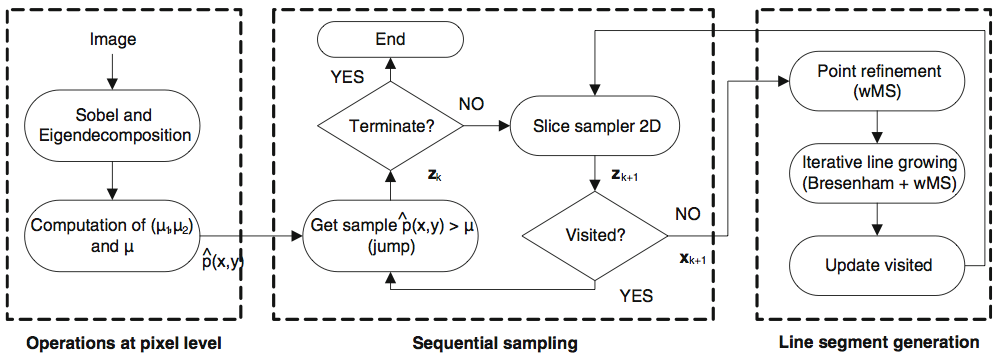
\includegraphics[width=\textwidth]{images/lswms} 
\caption{Ablaufschema des LSWMS Algorithmus. Im ersten Teil wird die Wahrscheinlichkeitsverteilung $\hat{p}(x,y)$ anhand der Parameter $\mu_1$ und $\mu_2$ ermittelt. Im zweiten Teil wird das erste Sample generiert und der Slice-Sampling-Prozess wird gestartet, um kontinuierlich Stichproben $z_k$ zu erhalten. Im dritten und letzten Teil werden die Samples verfeinert und als Ausgangspunkte für das iterative Line-Growing verwendet, welches die gesuchten Liniensegmente liefert. Quelle \cite{nieto}}
\label{fig:lswms}
\end{figure}
\noindent
Abb. \ref{fig:lswms} veranschaulicht den Ablauf des "Line Segment detection using Weighted Mean-Shift" (LSWMS) Algorithmus. Im ersten Teil wird die Wahrscheinlichkeitsverteilung für jedes Pixel von Bild $I$ berechnet, so dass $\hat{p}(x, y)$ angibt, wie wahrscheinlich es ist, dass das Pixel $(x, y$) Teil eines Liniensegmentes ist. Diese Wahrscheinlichkeitsverteilung, parametrisiert durch $\mu_1$ und $\mu_2$, wird anhand der Tensor Matrix und den dazugehörigen Eigenvalues errechnet. Gute Kandidatenpixel müssen zwei Bedingungen erfüllen. Zum einen muss der Betrag des Gradienten auf eine gewisse Signifikanz des Pixels hindeuten und zum anderen muss eine dominante Gradienten-Richtung in der Nachbarschaft des Pixels vorhanden sein.
\paragraph{}
Der zweite Teil \textit{sequential sampling} selektiert, basierend auf $\hat{p}(x,y)$, kontinuierlich Pixel ($z_k$) welche eine hohe Wahrscheinlichkeit besitzen zu einem Liniensegment zu gehören. Gleichzeitig wird sichergestellt, dass kein Pixel eines Segmentes mehrmals gesampelt wird. Dies ist ein wichtiger unterschied zu PHT, da es die Effizienz von LSWMS im Vergleich zu PHT erhöht. Der Slice Sampler basiert auf dem Markov-Chain-Monte-Carlo-Verfahren\footnote{\protect\url{http://de.wikipedia.org/wiki/MCMC-Verfahren}}, welches es erlaubt kontinuierlich Stichproben aus einer bestimten Wahrscheinlichkeitsverteilung $p$ zu ziehen, welche in unserem Fall die Qualität des Kandidatenpixel angibt.
\paragraph{}
Die Wahrscheinlichkeitsverteilung wird beim LSWMS Algorithmus anhand der Eigenvalues $(\lambda_1, \lambda_2)$ eines jeden Pixel berechnet. Wobei $f$ die Eigenvalues $(\lambda_1, \lambda_2)$ zu einem beliebigen Pixel $(x, y)$ zurückgibt.

\begin{equation}
\begin{split}
p = g \circ f:  &I \to (\lambda_1, \lambda_2) \to \mathbb{R} \\
                &(x, y) \mapsto \hat{p}(x, y) = g(f(x, y))
\end{split}
\end{equation}
\noindent
Die Funktion erfüllt zwei wichtige Kriterien. Zum einen gibt sie nur hohe Werte zurück für Eigenvalues-Paare bei dem ein Wert deutlich grösser ist als der andere. Zum anderen fällt der Wert rapide ab, wenn beide Werte hoch oder tief sind. $g$ gibt die Wahrscheinlichkeit an, dass ein Eigenvalue-Paar zu einem Liniensegment gehört.

\begin{equation}
g(\lambda_1, \lambda_2) = (1 - exp(-\lambda_1/\mu_1)) exp(-\lambda_2/\mu_2)
\end{equation}
\noindent
$\mu_1$ und $\mu_2$ sind die Durchschnittswerte aller Eigenvalues über das ganze Bild. Diese wurden im ersten Teil ermittelt. Stellt man die Verteilung visuell dar, so ergibt sich das Bild in Abb. \ref{fig:lswms-eigenvalues}.

\begin{figure}[!ht]
\centering
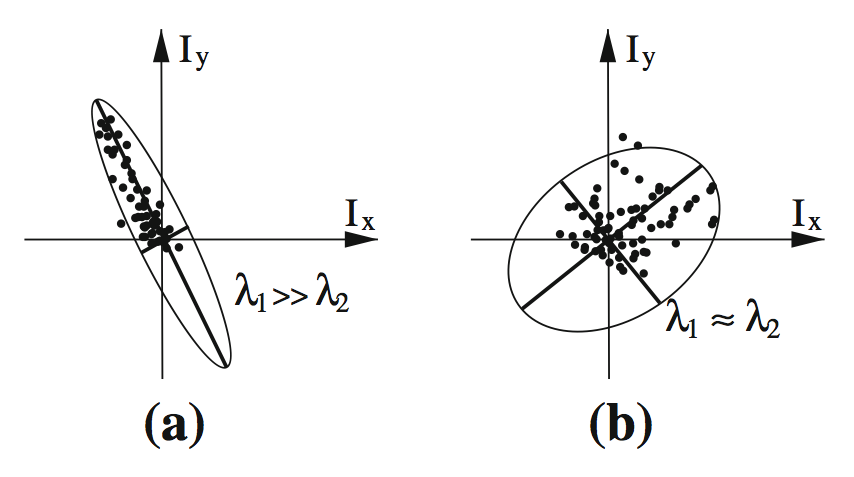
\includegraphics[width=\textwidth]{images/lswms-eigenvalues} 
\caption{Eigenvalues welche die Gradientenstruktur abbilden. Die schwarzen Punkte sind die Werte der Nachbarpixel eines Pixels $(I_x, I_y)$. a) Verteilung eines Liniensegmentes. b) Verteilung einer Ecke oder einer heterogenen Gradienten. Quelle \cite{nieto}}
\label{fig:lswms-eigenvalues}
\end{figure}
\noindent
\paragraph{}
Basierend auf diesen Grundlagen werden die Liniensegmente wie folgt ermittelt. Initial wird iterativ ein erster Kandidatenpixel gesucht, welcher die Bedingung $\hat{p}(x, y) > \mu$ erfüllt. $\mu$ ist der Mittelwert von $\hat{p}(x, y)$ über das ganze Bild. Dies stellt sicher, das für den Schritt der Segmentgenerierung eine optimale Ausgangslage geschaffen wird. So gibt es so wenig Fehlversuche wie möglich. Nachfolgend such der Sampler Pixel mit einem ähnlichen Wert für $\hat{p}(x, y)$ wie der Initialpixel. Jedes mal wenn ein Liniensegment generiert wird, werden sämtliche Pixel des Segmentes aus dem Pool der Pixel aus dem der Sampler wählt entfernt. Auch, werden die Nachbarpixel innerhalb einer definierten Fensters von $r x r$ entfernt, wobei r die räumliche Weite des Mean Shift ist. Aufgrund dieser Tatsache kann der Fall eintreten, dass der Slice Sampler feststellt, dass alle Pixel in der Nachbarschaft des initialen Pixels bereits verarbeitet wurden. In diesem Fall wird ein neuer Initialpixel gesucht, welcher die gegebenen Kriterien erfüllt. Der Sampler sucht so lange nach neuen Kandidaten bis keine geeigneten mehr gefunden werden oder bis eine gegebene Obergrenze bei der Anzahl zu suchender Liniensegmente erreicht wurde.
\paragraph{}
Die geeigneten Bildpunkte welche vom Slice Sampler ermittelt werden, werden kontinuierlich dem Line Segment Generator übergeben. Erhält dieser ein Sample $z_k$ und die dazugehörige Orientierung der Normalen $\theta_k$, so steuert er die Richtung des Generierungsprozesses anhand des Vektors $\textbf{x}_{k} = (x_k, y_k, \theta_k)$. Obwohl der Sampler bereits sehr gute Kandidaten liefert, besteht immer noch die Möglichkeit, dass in der Nachbarschaft von $\textbf{x}_k$ ein Bildpunkt mit einem höheren Wert für $\hat{p}(x, y)$ vorhanden ist. Aus diesem Grund wird mittels Weighted Mean Shift (wMS) nach einem Optimum $\hat{\textbf{x}}_k$ gesucht. Mean Shift (MS) ist ein iterativer, parameterfreier Algorithmus, welcher dazu eingesetzt werden kann lokale Maxima einer unbekannten Dichtefunktion zu ermitteln, wenn eine Menge von Samples vorhanden ist. Bei jeder Iteration startet MS bei einer initialen Stichprobe und bewegt sich in Richtung der dichtesten Region innerhalb des Suchraumes. LSWMS gewichtet die Stichproben zusätzlich noch anhand der zuvor berechneten Wahrscheinlichkeiten $\hat{p}$.
\paragraph{}
Anhand des verfeinerten Punktes $\hat{\textbf{x}}_k = (\hat{x}_k, \hat{y}_k, \hat{\theta}_k)$ wird dann die Generierung des Segmentes vorgenommen, basierend auf dem Bresenham Algorithmus \cite{bresenham}. Das obere Segment in der Abb. \ref{fig:lswms-line-growing}a veranschaulicht diesen Vorgang.

\begin{figure}[!ht]
\centering
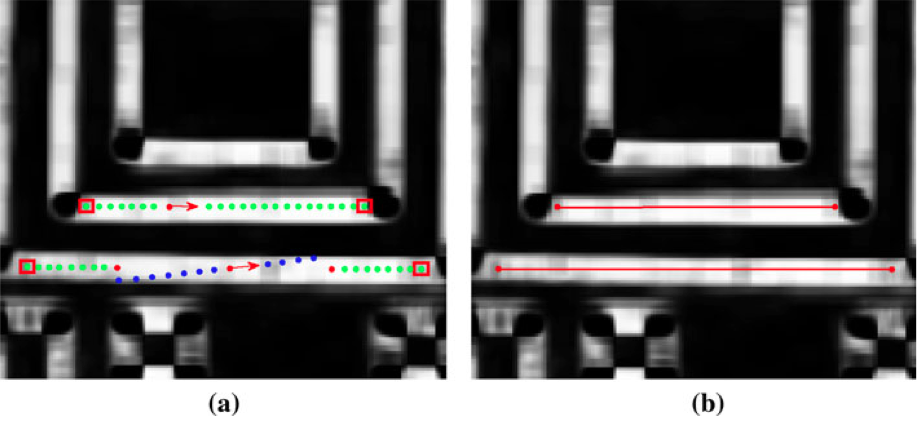
\includegraphics[width=\textwidth]{images/lswms-line-growing} 
\caption{Oriented Line Growing. a) Oberes Segment mit einer genauen Wachstumsrichtung. Unteres segment mit einem Wachstumsprozess welcher eine Verfeinerung der Richtung benötigt. b) In beiden Fällen wurde ein korrektes Segment ermittelt, welches sich innerhalb des Gradienten der Kante befindet. Quelle \cite{nieto}}
\label{fig:lswms-line-growing}
\end{figure}

\subsection{Evaluation}

Die Entscheidung fiel auf den LSWMS Algorithmus, aus mehreren Gründen. LSWMS wurde von Anfang an für die unbeaufsichtigte Kantendetektion innerhalb von Echtzeitanwendungen konzipiert. Da die Umgebungen in denen die Türdetektion stattfindet stark variieren können, ist es nicht möglich im vorhinein fixe Parameter für die Hough-Transformation zu definieren, welche überall gleich gut funktionieren. LSWMS bietet im Schnitt unter sich verändernden Verhältnissen die bessere Leistung. Der Algorithmus erforder zwar auch einen Parameter r, welcher oben erklärt wurde, jedoch kann dieser auf dem Standardwert 3 belassen werden. Mit diesem gibt LSWMS akzeptable Resultate zurück.
\paragraph{}
Ein weiterer Faktor ist die Qualutät der zurückgegebenen Resultate. Die Anzahl fehlerhaft erkannten Kanten ist bei Hough erheblich höher als bei LSWMS und wirkt sich damit auch auf die Performance der weiteren Verarbeitungsschritte negativ aus. Die Möglichkeit bei LSWMS eine Obergrenze bezüglich der Anzahl erwarteter Treffer angeben zu können war ebenfalls ausschlaggebend. Bei "ruhigen" Bildern mit wenig potentiellen Kanten wirkt sich dies wenig aus. Bilder welche z.B. Türe mit Holzmuster enthalten führen bei Hough zu einer Fehlerquote von teilweise über 50\%.
\paragraph{}
Der letzte Faktor welcher zur Entscheidung geführt hat LSWMS vorzuziehen war die Gesamtperformance. Hough benötigt als Input ein Kantenbild, welches zuvor mit einem separaten Algorithmus aufgearbeitet werden muss, z.B. Canny\footnote{\protect\url{http://de.wikipedia.org/wiki/Canny-Algorithmus}}. Dieser Schritt führt zusätzliche Parameter ein, welche situationsbedingt optimiert werden müssen und erhöht die Verarbeitungszeit der Hough-Transformation. Da Canny empfindlich gegenüber Rauschen im Bildmaterial ist, muss ein weiterer Verarbeitungsschritt vorangestellt werden. Bevor Canny angewendet wird, werden mittels einem Gausschen Filter Störfaktoren reduziert. Um ein optimales Ergebnis zu erhalten müssen vertikale und horizontale Kanten separat gesucht werden. Dies hat zu folge das die Hough-Transformation zweimal dürchgeführt werden muss (Canny muss nur einmal angewendet werden, beide Male kann das selbe Kantenbild verwendet werden).
\paragraph{}
Für den Vergleich der Hough-Transformation und LSWMS wurden folgende Parameter verwendet:
\paragraph{}
Gauss Filter (medianBlur)\footnote{\protect\url{http://docs.opencv.org/modules/imgproc/doc/filtering.html?highlight=medianblur#medianblur}}
\begin{itemize}
	\item kSize: 5
\end{itemize}
Canny Edge Detection\footnote{\protect\url{http://docs.opencv.org/doc/tutorials/imgproc/imgtrans/canny_detector/canny_detector.html}}
\begin{itemize}
	\item lowThreshold: 20
	\item highThreshold: 80
	\item kernelSize: 3
\end{itemize}
Probabilistic Hough Transform\footnote{\protect\url{http://docs.opencv.org/doc/tutorials/imgproc/imgtrans/hough_lines/hough_lines.html}}
\begin{itemize}
	\item rho: 1
	\item theta: 1 rad
	\item threshold: 80
	\item minLinLength: 30
	\item maxLineGap: 10
\end{itemize}
LSWMS
\begin{itemize}
	\item numMaxLSegs: 1000
\end{itemize}
\noindent
Die gelben Linien stellen die gefundenen Kanten bzw. Kanstensegmente dar.
\pagebreak

\begin{figure}
\subfloat[Ergebnis Hough-Transformation]{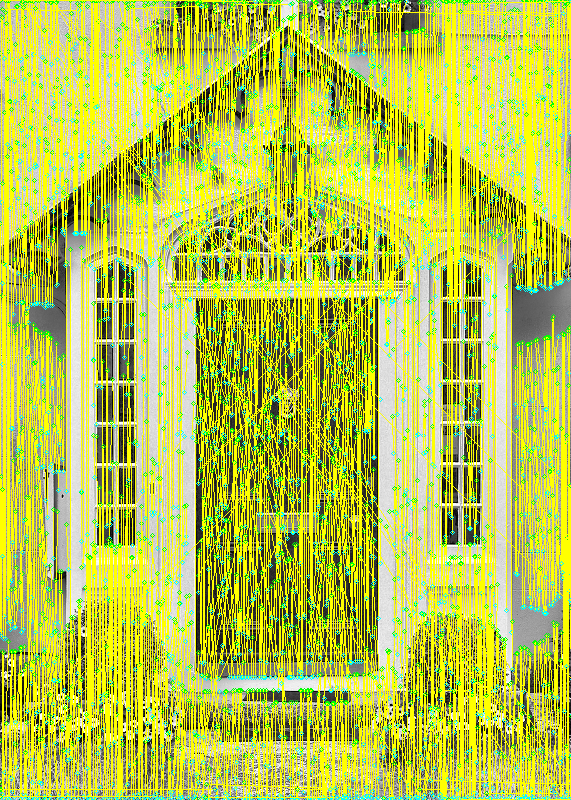
\includegraphics[width=0.47\textwidth]{images/hough-raw-segments}}\qquad
\subfloat[Ergebnis LSWMS]{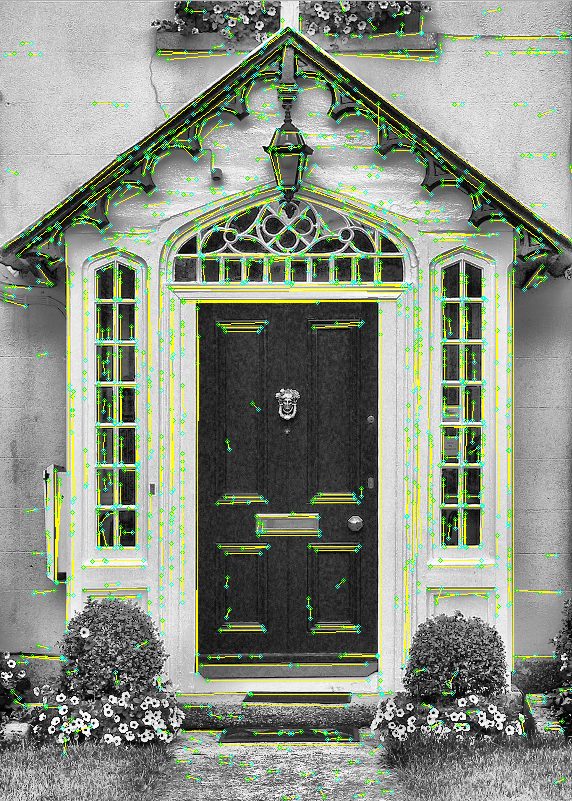
\includegraphics[width=0.47\textwidth]{images/lswms-raw-segments}}
\caption{Vergleich PHT und LSWMS}
\label{fig:comp-pht-lswms}
\end{figure}
\noindent
Dies ist nur ein Bild von zehn getesteten. Die Bilder welche während der Entwicklung zum Testen verwendet wurden können im Projektverzeichnis unter Data/Images/Doors/Misc gefunden werden. Es ist klar ersichtlich, dass LSWMS das qualitativ bessere Ergebnis liefert. Einziger Nachteil hier ist, dass LSWMS oft nicht durgehende Kanten erkennt sondern kleinere Segmente entlang der Kante zurückgibt. Neben der Qualität der Resultate wurde auch die Performance beider Methoden analysiert. Da einige Testbilder grösser sind als in der finalen Applikation benötigt, wurden alle Bilder auf eine Höhe von 800 Pixel verkleinert. Nachfolgend das Ergebnis (Durchschnitt aus 100 Durchgängen):

\begin{itemize}
	\item Hough: 165ms, 1871 Segmente
	\item LSWMS: 64ms, 868 Segmente
\end{itemize}
\noindent
Auch hier ist LSWMS Hough überlegen. Obwohl LSWMS für Echtzeitanwendungen konzipiert wurde, kann mit den gemessenen 64ms Verarbeitungszeit pro Frame kein flüssiges Videobild bei 28fps wiedergegeben werden.

\section{Implementation}

\begin{figure}[!ht]
\centering

\includegraphics[width=\textwidth]{images/door-detection} 
\caption{Ablauf der Türerkennung}
\label{fig:door-detection}
\end{figure}
\noindent
Wie bereits zu beginn des Kapitels erwähnt, besteht der Prozess der Türerkennung aus mehreren Teilschritten (Abb. \ref{fig:door-detection}). Als erstes wird der LSWMS Algorithmus angewendet. Dieser Arbeitet auf Graustufenbildern. Somit wird der Input entsprechend konvertiert. Da die Lichtverhältnisse vor allem an den Türkanten oft suboptimal sind, aufgrund eines leichten Schattenwurfes, wird eine Contrast Limited Adaptive Histogram Equialization (CLAHE) angewendet mit einem Clip Limit von 5 und einer Fenstergrösse von 8. Diese Werte wurden experimentell ermittelt. Der Grund, dass CLAHE angewendet wurde und keine normale (Adaptive) Histogram Equalization ist, dass festgestellt wurde, dass die Verstärkung von Rauschen und von feinen Muster (z.B. Holzmaserungen) die Qualität der Resultate von LSWMS verringert. Weiterhin ist es wichtig, dass die Regionen um die Tür herum ausgebessert werden. Dies ist damit gegeben, dass CLAHE den Kontrast immer innerhalb eines bestimmten Fensters ausgleicht. Um sichtbare Kanten der einzelnen Fenster zu vermeiden, wird die Randregion noch interpoliert. Der Unterschied der globalen Histogram Equalization und CLAHE wird in Abb. \ref{fig:clahe} verdeutlicht. Ein Beispiel wie die Ausgabe der LSWMS Erkennung aussieht, ist in Abb. \ref{fig:lswms-output} ersichtlich. Der Algorithmus wurde zusätzlich noch für diese spezielle Anwendung optimiert. Zu kurze Segmente werden bereits bei der Suche verworfen. Weiterhin wurde der Mean Shift teil entfernt. Dieser dient rein der Fehlerkorrektur. LSWMS gibt aber auch ohne diese Berechnung gute Resultate zurück. Der Mean Shift ist der Rechenintensivste Teil des Algorithmus. Durch den Ausbau konnte die Verarbeitungszeit um 70\% reduziert werden. Nur so konnte der oben genannte, deutliche Performancegewinn gegenüber PHT erreicht werden.

\begin{figure}
\subfloat[Ausgangsbild]{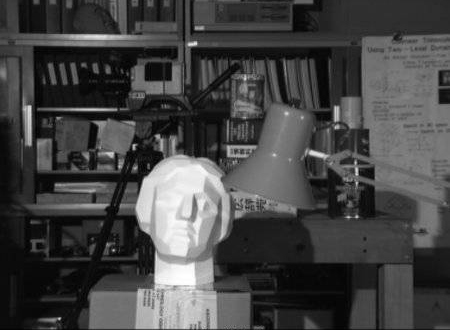
\includegraphics[width=0.47\textwidth]{images/clahe-orig}}\qquad
\subfloat[Global Histogram Equalization]{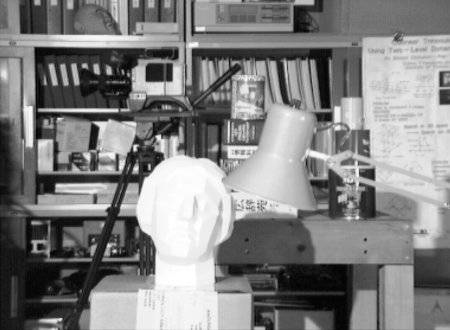
\includegraphics[width=0.47\textwidth]{images/clahe-ghe}}\qquad
\subfloat[Contrast Limited Adaptive Histogram Equialization]{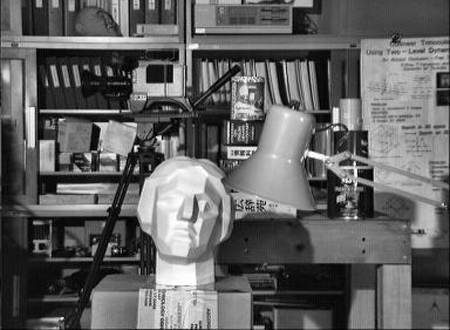
\includegraphics[width=0.47\textwidth]{images/clahe}}\qquad
\caption{Vergleich Global Histogram Equalization und CLAHE}
\label{fig:clahe}
\end{figure}

\begin{figure}
	\subfloat[Segmente wie sie von LSWMS gefunden werden]{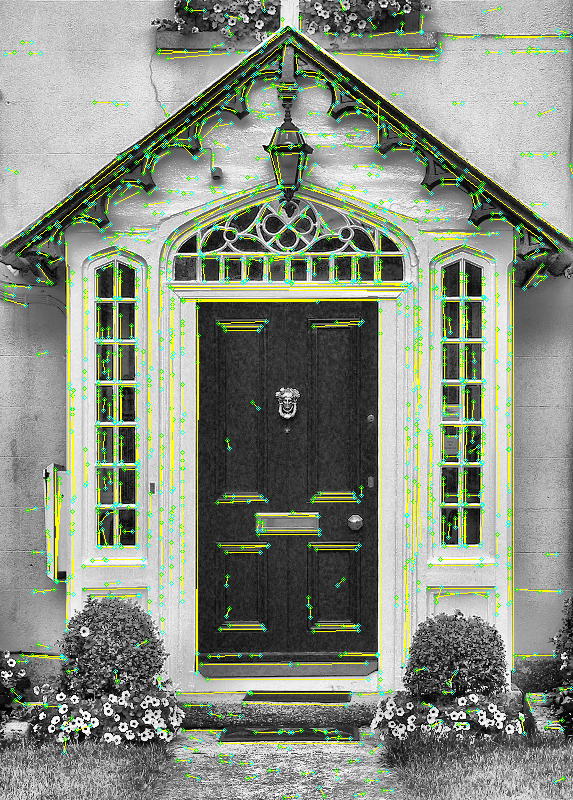
\includegraphics[width=0.45\textwidth]{images/seg-raw}\label{fig:lswms-output}}\qquad	
	\subfloat[Segmente kategorisiert in horizontal (Rot) und vertikal (Gelb)]{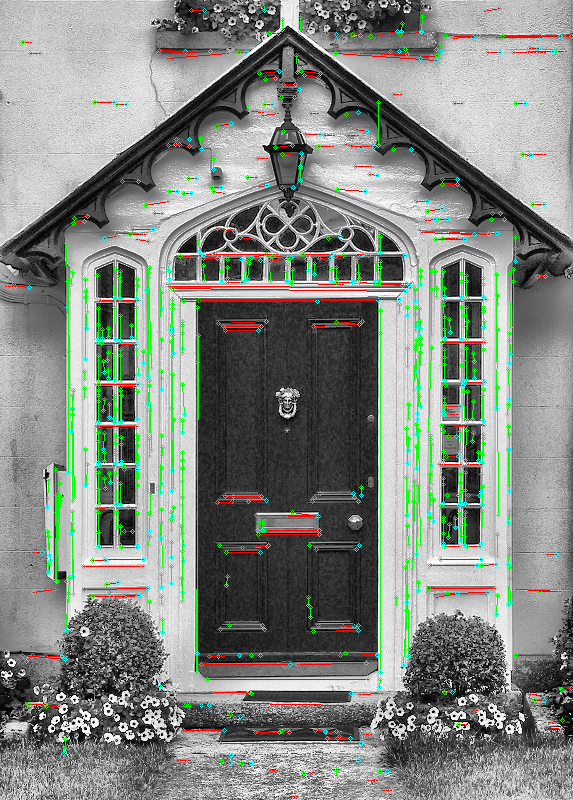
\includegraphics[width=0.45\textwidth]{images/seg-categorized}\label{fig:segs-categorized}}\qquad	
	\subfloat[Verschmolzene Segmente]{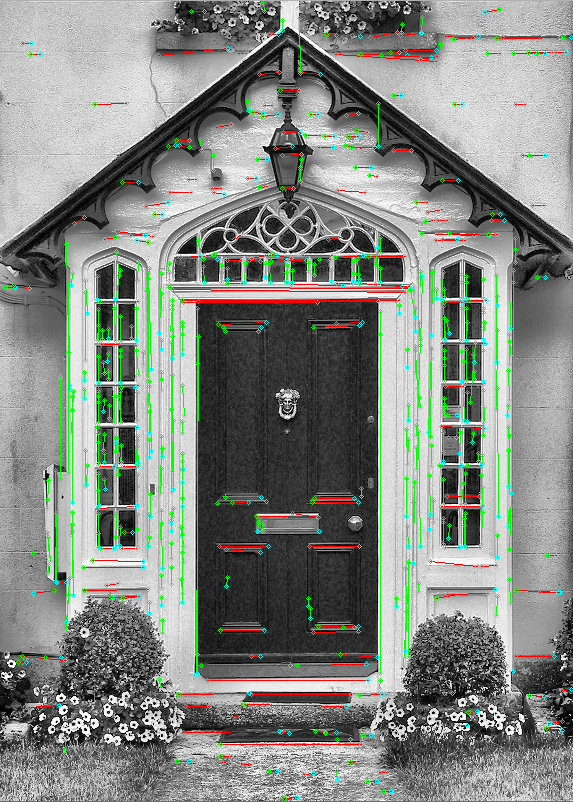
\includegraphics[width=0.45\textwidth]{images/seg-joined}}	\qquad	
	\subfloat[Verlängerte Segmente]{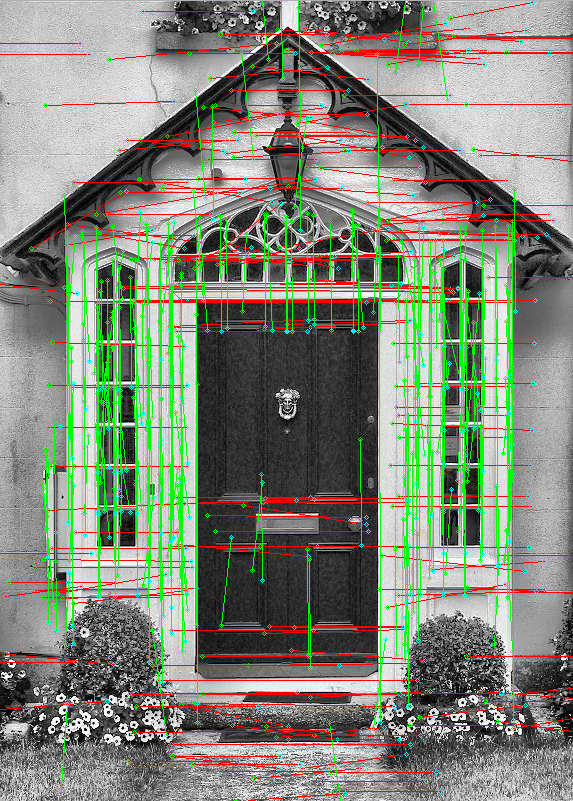
\includegraphics[width=0.45\textwidth]{images/seg-grow}}	
	\caption{Verarbeitungsprozess Türerkennung}
\end{figure}

\begin{figure}
	\ContinuedFloat
	\centering		
	\subfloat[Gefundene Kandidaten]{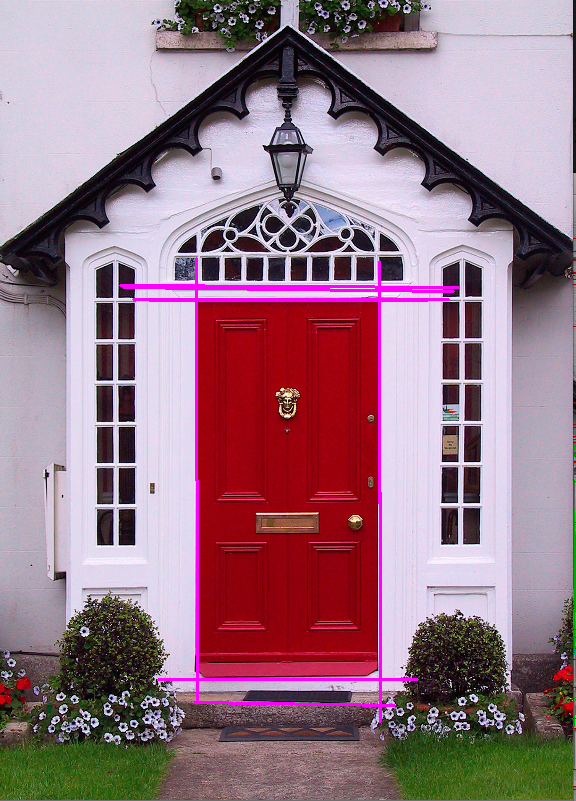
\includegraphics[width=0.45\textwidth]{images/seg-candidates}\label{fig:seg-candidates}}\qquad
	\subfloat[Erkannte Tür]{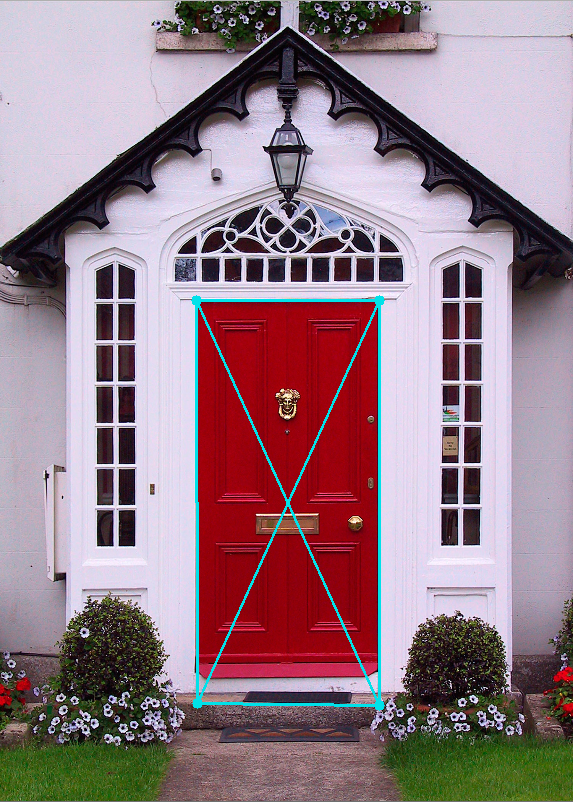
\includegraphics[width=0.45\textwidth]{images/seg-detected}}\qquad
	\caption{Verarbeitungsprozess Türerkennung}
	\label{fig:door-detection}
\end{figure}

\subsection{Kategorisierung}
Im nächsten Schritt werden die gefundenen Liniensegmente nach ihrer Ausrichtung kategorisiert (Abb. \ref{fig:segs-categorized}). Hierzu muss zuerst bestimmt weren, was horizontal und vertikal ist. Wird die Türe frontal aufgenommen, so sind  die gewohnten Werte $0$ für horizontal und $\frac{\pi}{2}$ für vertikal. Nimmt man die Türe seitlich auf, so wird vor allem die Horizontale verzerrt. Um nun zu bestimmen welcher Winkel der Ausgangspunkt für die Horizontale ist, werden bestimmte Annahmen getroffen. Horizontale Linien weichen auch bei einer starken seitlichen Aufnahme nie mehr als 50° (0.839rad) von der unverzerrten Horizontale ab. Für die Vertikale wurde ein Wert von 20° (0.3491rad) festgelegt. Diese Werte wurden aus Probeaufnahmen aus verschiedenen Winkeln ermittelt und sind in Source/Ardoor/DoorDetection/DoorDetector.hpp in den Konstanten MAX\_HORIZONTAL\_DIVERGENCE bzw. MAX\_VERTICAL\_DIVERGENCE festgehalten. Da nur längere Segmente verlässliche Informationen bezüglich der Ausrichtung liefern, wird eine Mindestlänge von 10\% der Diagonalen vorrausgesetzt. Alle Längenangaben bei der Türerkennung sind anhand prozentualer Anteile gegenüber der Diagonalen festgelegt, da die Diagonale die längst-mögliche Strecke in jedem Bild ist. So sind die Vorraussetzungen für jede Bildgrösse die selben. Wurden die Grenzwerte ermittelt, werden die Segmente nun kategorisiert. Hier wird eine Abweichung von 15° (MAX\_GRADIENT in Source/Ardoor/DoorDetection/LineSegment.hpp) zur Vertikalen bzw. Horizontalen erlaubt, um Fehler bei der Liniensegment-Erkennung auszugleichen und um eine bessere Grundlage für den nächsten Verarbeitungsschritt zu schaffen.

\subsection{Segment Joining}
Da die gefundenen Kanten oft nicht aus durchgehenden Segmenten bestehen sondern aus mehreren kleinen (Abb. \ref{fig:segments-pre-join}), müssen in diesem Schritt Liniensegmente die nahe bei einander liegen und eine änhliche Ausrichtung haben verschmolzen werden. Dabei wird wie folgt vorgegangen. Als erstes wird die Distanz der Segmente berechnet. Dabei müssen mehrere Fälle unterschieden werden.

\begin{itemize}
	\item Segmente sind parallel $\Rightarrow$ Die Distanz kann von jedem Punkt aus in der "Überlappungszone" bestimmt werden kann.
	\item Segmente stehen schief zueinander $\Rightarrow$ Die Segmentpunkte mit der geringsten Distanz müssen ermittelt werden.
	\item Segmente haben keine "Überlappungszone" $\Rightarrow$ Distanz von End- zu Startpunkt wird berechnet
	\item Segmente kreuzen sich $\Rightarrow$ Schnittpunkt muss ermittelt werden
\end{itemize}

\begin{figure}[!ht]
\centering
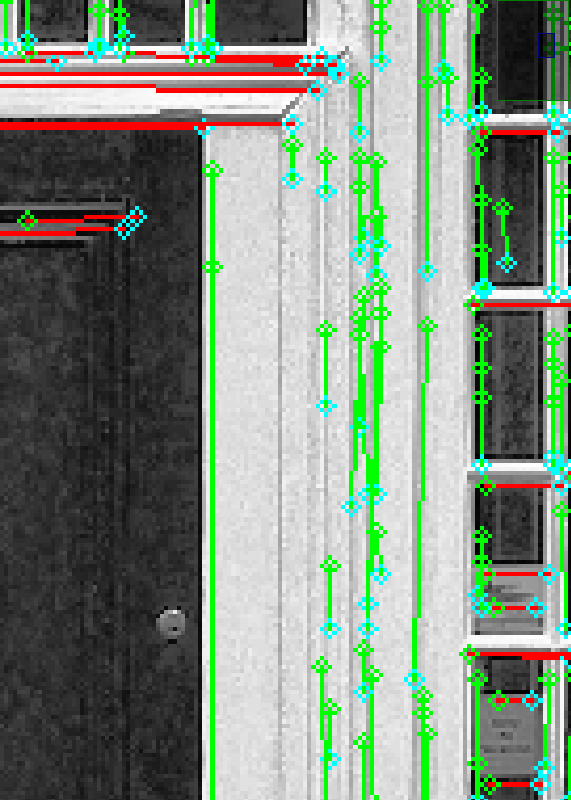
\includegraphics[width=0.5\textwidth]{images/segments-pre-join} 
\caption{Segmente vor der Verschmelzung (gezoomt)}
\label{fig:segments-pre-join}
\end{figure}
\noindent
Eine Distanz von max. 8px hat sich als guter Wert erwiesen. Wurden zwei Segmente gefunden die nahe genug beieinander sind, wird das Segment Joining initialisiert. Hier wird zuerst überprüft, ob es Sinn macht die Segmente zu vereinen. Liegt ein Segment innerhalb des Bereiches des anderen, so macht dies keinen Sinn, da das Segment nicht erweiter wird (Abb. \ref{fig:segment-joining-1}).

\begin{figure}[!ht]
\centering
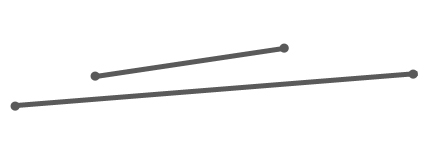
\includegraphics[width=0.5\textwidth]{images/segment-joining-1} 
\caption{Hier macht es keinen Sinn die zwei Segmente zu verschmelzen}
\label{fig:segment-joining-1}
\end{figure}
\noindent
Ist dies nicht der Fall, so wird ermittelt, welches Segment die bessere Ausrichtung gegenüber der errechneten Horizontalen bzw. Vertikalen hat. Die bessere Ausrichtung wird beim Verbinden beibehalten. Anschliessend werden die Längen addiert und das neue Segment wird zwischen den zwei Ausgangssegmenten platziert (Abb. \ref{fig:segment-joining-2}).

\begin{figure}[!ht]
\centering
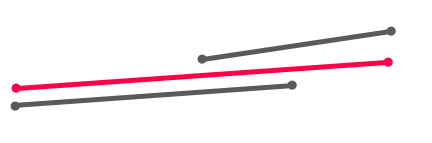
\includegraphics[width=0.5\textwidth]{images/segment-joining-2} 
\caption{Ausgangssegmente grau und verschmolzenes Segment rot}
\label{fig:segment-joining-2}
\end{figure}

\subsection{Kandidatensuche}
Nun gehr es darum Vierer-Paare von Liniensegmenten zu finden, welche eine Tür darstellen könnten (Abb. \ref{fig:seg-candidates}). Währen der Implementation der Suche hat sich ergeben, dass die Segmente welche die Tür umgeben sich nicht kreuzen. Aus diesem Grund werden die Linien vor der Suche noch um 5\% der Diagonalenlänge verlängert. Mit diesem Wert konnte in allen Tests sichergestellt werden, dass sich die Türsegmente überlappen. 
\paragraph{}
Nun wird nach der Tür gesucht. Hierfür werden als erstes die vertikalen Kanten evaluiert. Diese müssen einen gewissen Mindestabstand besitzen (15\% der Diagonallänge). Damit gehen wir davon aus, dass die Tür an sich im Bild eine gewisse Grösse hat. Dies lässt sich nicht vermeiden, um nicht fälschlicherweise Fenster als Türen zu erkennen. Anschliessen wird nach passenden horizontalen Segmenten gesucht. Diese müssen min. eine Türhöhe von 25\% bilden. Es werden nur die horizontalen Linien evaluiert, welche beide vertikalen Segmente überlappen.

\subsection{Kandidatenevaluation}
In diesem letzten Schritt werden die gefundenen Kandidaten bewertet. Dabei wird das Seitenverhältnis Höhe zu Breite von diesen ausgewertet. Es wurden verschidene Türtypen aufgenommen und im Internet gesucht um zu erruieren, was in etwa das Standardmass einer Durchschnitttür ist. Es sind zwar DIN-Normen vorhanden, diese weichen aber stark von den meisten Türen ab welche untersucht wurden. Die DIN-Norm für eine einflüglige Türe hat ein Seitenverhältnis von 7.2. Durch Auswertung von 30 Aufnahmen wurde aber ein Verhältnis von 4.91 errechnet. In den Tests hat sich dieses klar als besser herausgestellt in 100\% der Fälle. 
\paragraph{}
Es wurden auch diverse andere mögliche Evaluationskriterien getestet, jedoch haben sich diese nicht bewährt. Ein Ansatz war, die farbliche Homogenität der Fläche der Kandidaten zu bewerten. Aufgrund von Schattenwurf, Fenstern und Mustern auf vielen Türen hat sich dies nicht bewährt. Ein anderer Ansatz war, den Türgriff zu suchen. Da die Vielfalt hier aber enorm gross ist und der Griff oft zu klein ist auf den Bildern um ihn zu Analysieren, wurde auch dieses Kriterium fallen gelassen. Generell ist es sehr schwierig bei Aussentüren einen gemeinsamen Nenner zu finden. Die Evaluation der Seitenverhältnisse allein liefert aber in vielen Fällen bereits gute Resultate.

\subsection{Performance}
Die Performance wurde anhand von 100 Durchläufen auf 10 verschiedene Bilder gemessen.

\begin{itemize}
	\item \textbf{LSWMS} (inkl. CLAHE): 64ms
	\item \textbf{Kategorisierung} 0.02ms
	\item \textbf{Segment Joining} 1.05ms
	\item \textbf{Kandidatenevaluation} 9$\mu$s
\end{itemize}

\noindent
Wie zu sehen ist, ist nur der Teil der Kantendetektion für die Gesamtperformance relevant. 

\subsection{Verbesserungsmöglichkeit}
Zwei essentielle Punkte können an der Türerkennung verbessert werden. CLAHE ist eine vergleichsweise rechenintensive Operation. Ohne diese nimmt der LSWMS im Schnitt nur 23ms in Anspruch. Jedoch sind die Suchresultate deutlich schlechter ohne diese Kontrastoptimierung. Hier muss nach einer Alternative gesucht werden.
\paragraph{}
Ein zweiter Schwanchpunkt ist die Ermittlung der effktiven Horizontalen und Vertikalen. Bei starken Seitenaufnahmen mit einem Winkel von <70° sind die Abweichungen zu gross (Abb. \ref{fig:door-joining-error}). Hier muss der Fluchtpunkt ermittelt werden um die Zuverlässigkeit zu verbessern. Da das Ziel war die Performance auf Echtzeiniveau zu bringen, wurde versucht auf die Berechnung der Fluchtpunkte zu verzichten. Jedoch hat sich zum Schluss ergeben, dass dies wohl unumgänglich ist. Zeitlich konnte dies aber nicht mehr realisiert werden.

\begin{figure}	
\subfloat[Kanten vor dem Joining]{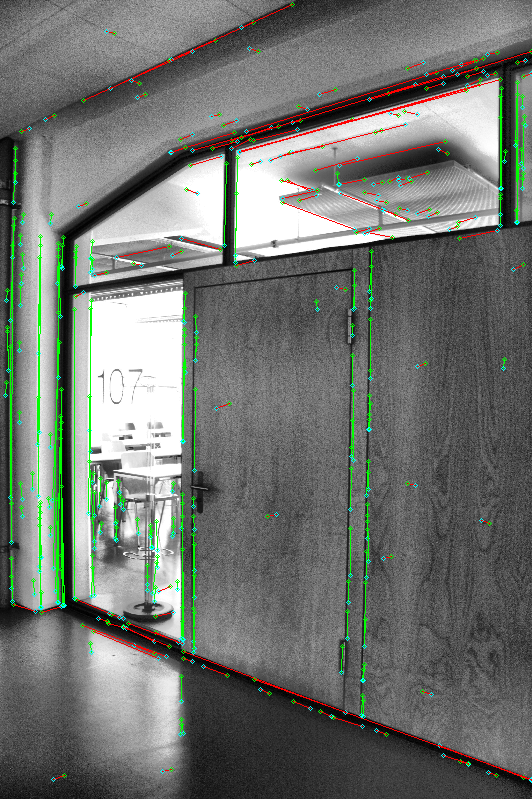
\includegraphics[width=0.48\textwidth]{images/door-side-raw}}\qquad
\subfloat[Kanten nach dem Joining]{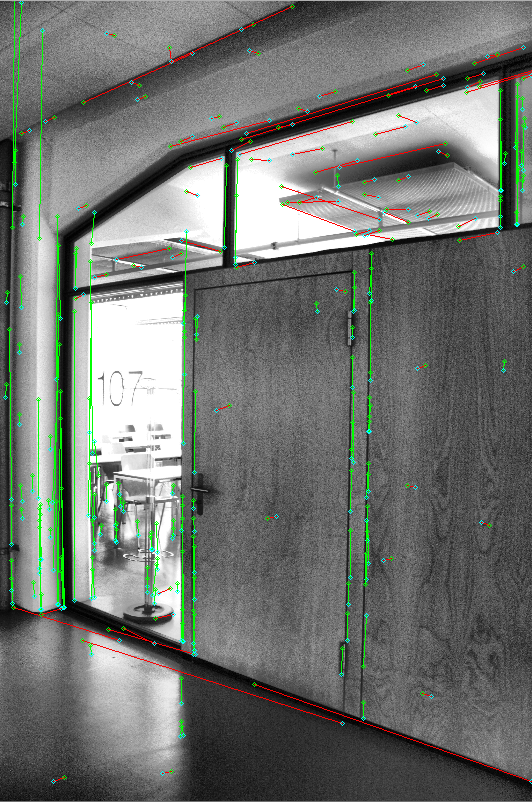
\includegraphics[width=0.48\textwidth]{images/door-side-joined}}\qquad
\caption{Abweichung bei der Bestimmung der Horizontalen. Die untere Türkante weicht nach dem Segment Joining klar von der effektiven Horizontalen ab.}%
\label{fig:door-joining-error}
\end{figure}
\newpage

%\chapter{Plattformunabhängigkeit}

In diesem Abschnitt werden die Details der Implementationen auf den beiden Smartphone-Plattformen iOS und Android, sowie den Aufbau unserer ARDoor Library beschrieben.

\section{Grundarchitektur}
Wir haben die Grundarchitektur unserer Applikation laut Abb. \ref{fig:android-architecture} definiert. Die einzelnen Komponenten werden hier kurz beschrieben.

\paragraph{OpenCV}
ist ein quasi-Standard in der nativen Bildverarbeitung und unterstützt eine Vielzahl an Bearbeitungsfunktionen. OpenCV wird in der ARDoor Library für die Bildverarbeitung verwendet.

\paragraph{OpenGL}
wird für das 3D-Rendering benötigt. In der mobilen Welt ist die Library mittlerweile Standard und wird von Android und iOS unterstützt.

\paragraph{ARDoor C++ Library}
Die ARDoor Library enthält den Hauptteil der Applikation. In ihr wird sämtliche plattformunabhängige Logik sowie Verarbeitung und Rendering implementiert. C++ eignet sich  dafür gut, da sowohl von iOS via Objective-C als auch von Android über JNI auf die Library zugegriffen werden kann.

\paragraph{Plattformspezifischer Client}
Pro Plattform wird ein eigener Client implementiert, der den Kamerazugriff übernimmt. Die erfassten Einzelbilder werden an die ARDoor Library zur verarbeitung weitergereicht. Dieser Client sollte nur als Zwischenschicht dienen und deshalb so schlank wie möglich gehalten werden. 


\begin{figure}[!ht]
\centering
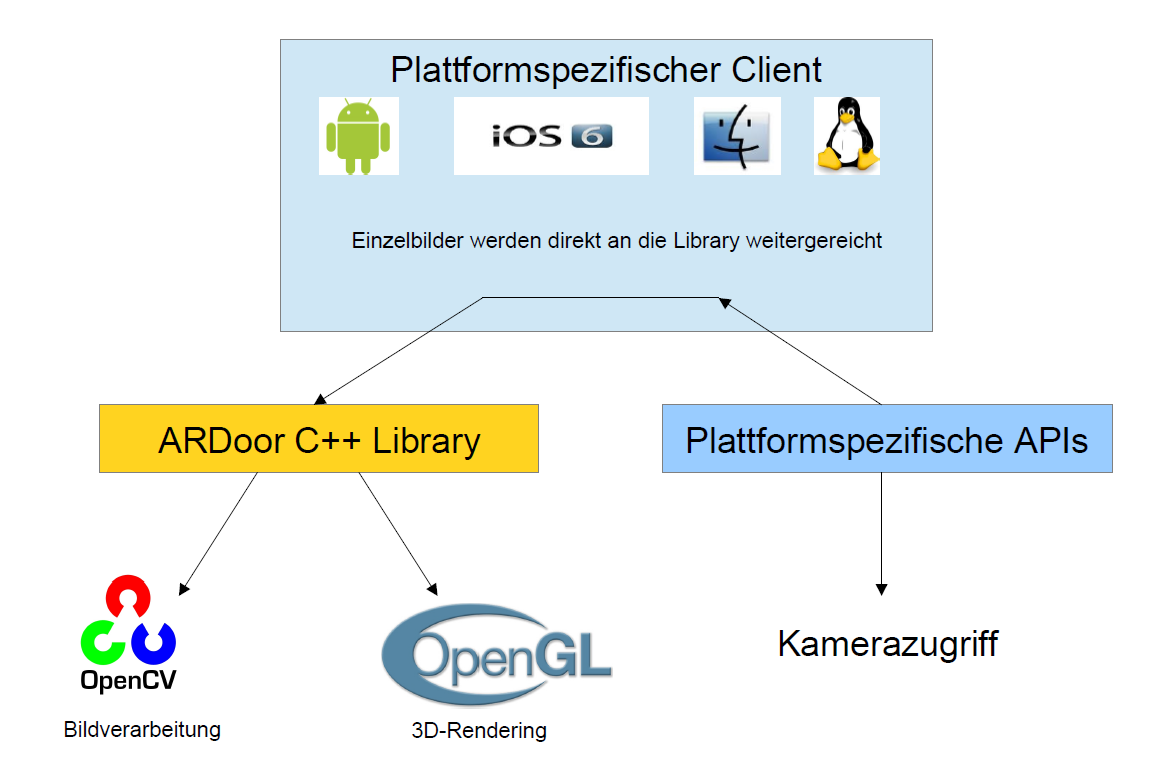
\includegraphics[scale=0.4]{images/architecture.png} 
\caption{Grundarchitektur von ARDoor}
\label{fig:android-architecture}
\end{figure}

\section{Android Plattform}
Zur Entwicklung und zum Testen unter Android wurde ein etwas in die Jahre gekommenes HTC Desire Z verwendet. Es wurde jedoch eine Custom Firmware aufgespielt, welche der Android Version 2.3 entspricht, um bessere Native-Unterstützung zu erhalten. Seit dieser Version, welche dem API Level 9 entspricht, gibt es u.a. die Möglichkeit, eine Native Activity zu implementieren.


\subsection{Native Activity}
Eine Native Activity ist seit Android 2.3 (API Level 9) verfügbar. Eine Native Activity ist im Grunde ein nützlicher Weg, um eine Android App in C/C++ zu implementieren, ohne noch zusätzlichen Wrapper-Code in Java und JNI Code zu schreiben. Mittels der dem Android NDK beiliegenden Library android\_native\_app\_glue kann das Grundgerüst der Native Activity in C/C++ implementiert werden. Dies hat jedoch einige Probleme bereitet.

\paragraph{}
Eines der Probleme war, dass primär zur Entwicklung unter Android Java (via Dalvik VM) als Programmiersprache vorgesehen ist. Ein Grossteil der verfügbaren APIs ist aus diesem Grund nur über Java aufrufbar. Dazu gehört auch die API für den Kamerazugriff. Es wäre zwar möglich aus C++ über JNI mit der Java-API zu kommunizieren, jedoch ist dies aufwändig und fehleranfällig. Auch verursacht JNI einen gewissen Overhead, wodurch ein Aufruf der rein in Java implementierten APIs aus Java-Code heraus schneller ist. JNI Code ist ausserdem sehr mühsam zum lesen und verursacht hohen Wartungsaufwand.

\paragraph{}
Es gibt auch die Möglichkeit mittels der OpenCV Capture-API auf die Kamera des Smartphone zuzugreifen. Das Problem dabei ist, dass OpenCV dazu nicht dokumentierte Funktionen aus einer Android System-Library aufruft. Dies funktioniert leider nicht mit allen Geräten. Da die aufgerufenen Funktionen nicht zu einer offiziellen, stabilen API gehören, können diese bei einer neuen Android-Version ändern und die Entwickler von OpenCV müssten diese Unterstützung zuerst implementieren.

\paragraph{}
Was bei der Native Activity auch beachtet werden muss ist, dass die ganzen Android-Events, z.B. Input oder App-Lifecycle-Events, selber abgeholt und weiterverarbeitet werden müssen. Dadurch schreibt man quasi von Grund auf ein eigenes Applikationsframework auf nativer Basis.


\subsection{JNI Zugriff}
Die andere Möglichkeit ist der Zugriff auf C/C++ via JNI. Die Grund-App wird dabei in Java implementiert. In der nativen Library werden bei dieser Methode spezielle JNI-Funktionen implementiert, die aus Java heraus aufgerufen werden können.

\paragraph{}
Bei dieser Variante haben wir zwar immer noch die Java-Schicht, jedoch kann dadurch auf eine stabile und funktionierende API zurückgegriffen werden. Auch ist es einfacher später ein GUI zu implementieren, z.B. zur Auswahl des zu projizierenden 3D-Models.


\section{iOS Plattform}
Zur Entwicklung der iOS Version der Applikation haben wir ein iPhone 4 eingesetzt welches einen A4 Prozessor basierend auf der ARMv7-A\footnote{\url{http://www.arm.com/products/processors/instruction-set-architectures}} Architektur besitzt. Die plattformspezifischen Funktionen wurde in Objective-C geschrieben. Im Gegensatz zu Android braucht es auf der iOS Plattform keine Bridge um C++ Code ausführen zu können. Da Objective-C wie auch C++ eine Obermenge von C ist, können C++ Klassen in der gewohnten Syntax direkt verwendet werden. Dies ist einer der grössten Vorteile der iOS Plattform. Fast alle bestehenden C und C++ Bibliotheken können ohne Umwege Verwendet werden.

\paragraph{}
Einen weiteren Vorteil welchen Objective-C bietet ist, dass alle Klassen grundsätzlich Beliebig erweitert werden können. So konnten wir z.B. die \textit{UIImage} Klasse um Funktionen erweitern, welche es uns ermöglichen den Inhalt eines \textit{UIImage} in eine \textit{cv::Mat} Struktur umzuwandeln und umgekehrt (zu Finden in der Klasse \textit{UIImage+OpenCV}). Somit gestaltete sich der Datenaustausch zwischen den plattformspezifischen Komponenten und unserer unabhängigen ARDoor Library sehr einfach.

\subsection{Kamerazugriff} Der Kamerazugriff ist eher etwas komplex gestaltet unter iOS. Glücklicherweise ist die Dokumentation von Apple sehr ausführlich und bietet zu allen komplexen Prozessen Codebeispiele. So auch für den Kamerazugriff. Dies hat uns einiges an Zeit gespart, denn ohne diese Beispiele muss man sehr tiefgehende Kenntnisse – ja man muss schon fast ein Experte sein – von iOS haben um den Kamerazugriff zu konfigurieren. Die Komponenten für Audio und Video In- und Output befinden sich im AVFoundation Framework Welches wiederrum CoreMedia und CoreVideo verwendet (Abb. \ref{fig:avfoundation}).

\begin{figure}[!ht]
\centering
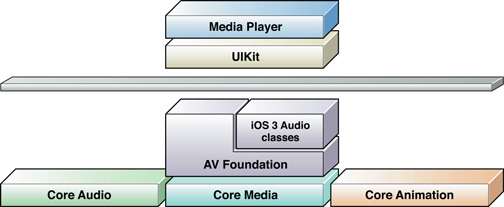
\includegraphics[scale=0.6]{images/avfoundation.jpg} 
\caption{Aufbau des Medienzugriffes unter iOS, Quelle: \protect\url{http://developer.apple.com/library/ios}}
\label{fig:avfoundation}
\end{figure}

Das Setup für den Kamerazugriff gestaltet sich dann wie folgt:

\begin{itemize}
\item Als erstes muss eine Instanz von \textit{AVCaptureDevice} aufgesetzt werden. Diese repräsentiert das Gerät über welches der Input geliefert wird.
\item Über eine \textit{AVCaptureDeviceInput} wird der Datenstrom des Eingabegerätes gesteuert.
\item Mittels \textit{AVCaptureVideoDataOutput} wird die Ausgabe der Daten, in unserem Fall auf ein UIImage, gesteuert.
\item Die letzte Komponente ist die \textit{AVCaptureSession}, welche den Datenstrom von \textit{AVCaptureDeviceInput} zu \textit{AVCaptureVideoDataOutput} steuert.
\end{itemize}

Der Afbau ist in Abb. \ref{fig:ios-capture-overview} visualisiert. Der Code für das Setup befindet sich in \textit{VideoCaptureViewController::createCaptureSessionForCamera}. Obwohl der Kamerazugriff eher komplex aufgebaut ist, bietet er auch einige vorteile. Es ist einfach mehrere Input-Devices wie eine Kamera und ein Mikrofon zusammenzufassen. Weiterhin kann man auch sehr einfach das Input-Device austauschen, z.B. die Backface-Kamera mit der Frontface-Kamera. Beides, ohne dass die darunterliegenden Layer etwas davon mitbekommen.

\begin{figure}[!ht]
\centering
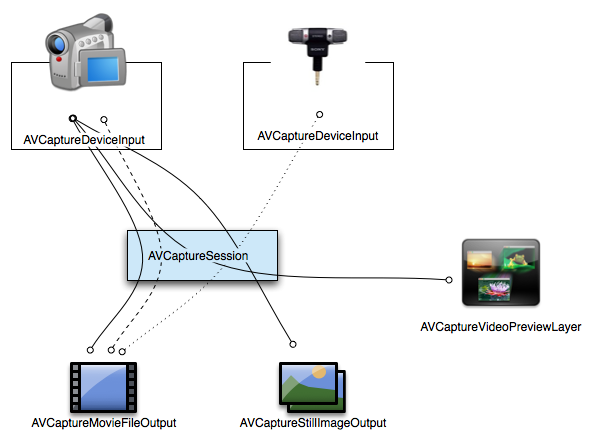
\includegraphics[scale=0.6]{images/ios-capture-overview.png} 
\caption{Aufbau des Medienzugriffes unter iOS, Quelle: \protect\url{http://developer.apple.com/library/ios}}
\label{fig:ios-capture-overview}
\end{figure}

\subsection{OpenCV unter iOS}
OpenCV lässt sich unter iOS mittlerweile sehr einfach einbinden. Noch bis vor kurzem musste man die Bibliothek noch selbst für die ARM-Plattform kompilieren, was sich als sehr mühsam erwies. Jedoch bieten die OpenCV-Macher mittlerweile vorkompilerte Binaries in Form eines Framework-Bundles an. Die Framework-Bundle Form hat den Grossen vorteil, dass die Binaries mit relativen Pfaden gelinkt sind. So ist das Deployment viel einfacher. Andernfalls müsste man nach der Kopilierung die Linker-Pfade mittels otool vor dem Deployment anpassen. Eine iOS App wird zuerst lokal auf dem Entwicklungsrechner Kompilert und danach auf das Endgerät (oder den iOS Simulator) installiert. Da die Verzeichnisstrukturen nicht auf beiden Geräten identisch ist, währen somit die Linker-Pfade nicht korrekt wenn sie absolut wären.

\paragraph{Performance} Die Performance von OpenCV unter iOS ist nicht optimal. Innerhalb von OpenCV wird standardmässig OpenMP für die Parallelisierung eingesetzt. Da jedoch OpenMP bisher noch nicht auf ARM portiert wurde, wird die Leistung des Prozessors nicht voll ausgeschöpft. So drückt eine Sobel-Live-Kantendetektion des Kamerabildes die Framerate bereits auf ca. 13 fps runter. Die Erkennung einen Schachbrettmusters mittels \textit{cv::findChessboardCorners} bringt es nicht einmal mehr auf ein fps. Eine Möglichkeit hier die Performance zu Optimieren währe Grand Central Dispatch (GCD) einzusetzen. Dies ist die Objective-C spezifische Multithreading Umgebung von Apple. Seit der Version 2.4.3\footnote{\url{http://code.opencv.org/projects/opencv/wiki/ChangeLog}} besitzt OpenCV eine \textit{parallel\_for} Implementierung für diverse Multithreading Backends, unter anderem auch für GCD. Eine weitere Möglichkeit die Leistung der Anwendung zu optimieren währe, wo möglich, Operationen mittels NEON\footnote{\url{http://www.arm.com/products/processors/technologies/neon.php}} umzusetzen. NEON ist ein SMID Instruction Set, ähnlich wie MMX von Intel, welches parallele Operationen auf einer Instruktion erlaubt. Beide Optionen gilt es während der Bachelor-Thesis zu erforschen.

\section{Desktop Platform}
Da die Performance von OpenCV auf den mobilen Geräten suboptimal ist und es auf Grund der tiefen Frameraten sehr mühsam wurde die Applikation zu testen, haben wir uns dazu entschieden auch eine Desktop-Variante umzusetzen. Als Grundlage dafür haben wir das QT-Framework eingesetzt. Zu begin haben wir auch noch eine Mac OS X spezifische App entwickelt. Jedoch wurde der Aufwand zwei Desktop Varianten zu entwickeln schlicht zu hoch, da wir uns in beide Plattformen zuerst tiefer einarbeiten hätten müssen. Deshalb haben wir uns dazu entschlossen, nur noch die QT-Variante weiterzuentwickeln. Mittels QT-Framework kann sowohl unter Mac OS X als auch unter Linux entwickelt werden, welche die Zielplattformen für die Desktop App waren. Einzig bei der Einbindung von Libraries wie OpenCV und bei der Einbindung von einigen Header-Dateien müssen Weichen für OS X und Linux eingebaut werden, da die Namensgebung nicht immer identisch ist. 
\paragraph{}
Eine wichtige Einstellung welche vorgenommen werden musste ist die Deaktivierung des QML-Debuggers. Solange diese Option aktiv war, wurde der eigentliche C++ Debugger nicht korrekt ausgeführt. Das führte dazu, dass Fehler im Code nicht erkannt werden konnten. Die Applikation verhielt sich nicht wie erwartet, gleichzeitig wurden beim Kompilieren aber keine Fehler ausgegeben; Breakpoint wurden einfach ignoriert. Weiterhin verhielt sich das Event-Handling innerhalb von QT nicht wie spezifiziert, solange der QML-Debugger aktiv war. Diese Situation führte zu einer erheblichen Verzögerung in der Entwicklung, bis dieser Konfigurationsparameter als Ursache lokalisiert wurde. Der Grund für dieses Fehlverhalten könnte sein, das wir nicht QML für die Erstellung des UI einsetzen, sondern das XML basierte System. Wahrscheinlich gibt es Inkompatibilitäten zwischen den zwei Libraries.
\paragraph{}
Ein weiteres Hindernis welches wir hatten war die Kompilierung von OpenCV unter Mac OS X. Leider bieten die Hersteller keine precompiled Binaries für Mac OS X an. Das Problem bestand darin, dass der Linker falsche relative Pfade zu OpenCV gesetzt hat. Erst als wir einen Patch für OpenCV\footnote{\url{http://code.opencv.org/issues/2037}} entdeckt hatten, welcher es erlaubte die Bibliothek als Framework zu verpacken, konnte OpenCV problemlos unter Mac OS X betrieben werden. Ein Problem welches bis heute noch ungelöst ist, ist die OpenGL-Unterstützung innerhalb von OpenCV unter Mac OS X. Obwohl der nötige Kompilierungsparameter \textit{WITH\_OPENGL} korrekt gesetzt wurde, wurde OpenCV ohne OpenGL-Unterstützung kompiliert. Dies führte dazu, dass wir viele Beispielapplikationen nicht Ausprobieren, da diese OpenGL-basierte GUIs verwenden.

\section{Calibration Dialog}
Der Calibration Dialog dient dazu, die Kameraparameter zu ermitteln. Dies muss grundsätzlich nur einmal zu Begin gemacht werden. Die gewonnenen Daten werden anschliessend in eine Konfigurationsdatei abgelegt. Die Datei wird im systemspezifischen Konfigurationsverzeichnis abgelegt.

\section{Mainwindow}
Das Mainwindow ist der Hauptteil der Applikation. Innerhalb von diesem wird die Augmented Reality Szene dargestellt.

\section{ARDoor Library}
Wir haben uns zum Ziel gesetzt, die ARDoor Library möglichst modular aufzubauen, so dass wir verschiedene Komponenten einfach austauschen könnten und wir somit flexibel in der Entwicklung sind. Da wir bei der Entwicklung sehr viele Dinge ausprobiert haben und ständig Sachen neu implementiert haben, konnten wir dies nicht zu 100\% umsetzen. Sobald wir eine erste funktionierende Version mit Positionsbestimmung und korrektem Rendering haben, werden wir ein generelles Code-Refactoring durchführen.

\section{ImagePipeline}
Eine der Hauptkomponente der ARDoor Library ist die Image Pipeline. Der Grundgedanke dahinter ist, dass die verschiedenen Schritte zur Bildbearbeitung und -verarbeitung in sich geschlossenen modularen Klassen - einem \textit{ImageProcessor} - implementiert werden. Wir erhoffen uns davon eine einfachere Entwicklung, da wir dadurch die verschiedenen Verarbeitungsschritte einfach austauschen oder in der Reihenfolge der Ausführung neu positionieren können.

\paragraph{}
Ein weiterer Grundgedanke für diesen Aufbau war, dass wir so einfach Debugmöglichkeiten einbauen könnten: Man könnte einen einfachen Debug ImageProcessor, der das aktuelle Bild nur darstellt und nicht verändert, implementieren und diesen an eine beliebige Position der Pipline setzen.

\paragraph{}
Implementiert haben wir die Pipeline so, dass für jedes Bild, welches wir von der Kamera erhalten, eine OpenCV-Matrix cv::Mat erzeugt wird. Diese wird der Pipeline nun zur Verarbeitung übergeben. Die Pipeline übergibt diese Matrix dem aktuellen ImageProcessor, der eine weitere Matrix als Rückgabewert liefert. Die zurückgegebene Matrix wird jeweils als Eingabe für den nächsten ImageProcessor in der Pipeline verwendet. Zum Schluss wird von der Pipeline das finale Bild nach allen Verarbeitungsschritten zurückgegeben. Dieser Ablauf ist in Abbildung \ref{fig:image-pipeline} grafisch dargestellt.

\begin{figure}[!ht]
\centering
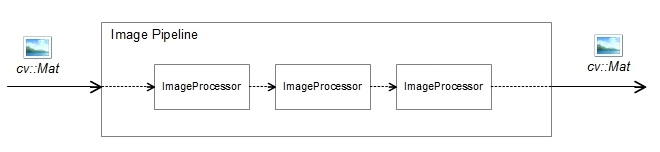
\includegraphics[scale=0.8]{images/image-pipeline.jpg} 
\caption{Aufbau der Image Pipeline}
\label{fig:image-pipeline}
\end{figure}

\section{RenderingContext}
Eine weitere Komponente der Library ist der RenderingContext. Die primäre Aufgabe dieser Komponente ist das Rendering der 3D-Modelle einer Szene sowie das korrekte setzen der Projektions- und ModelView-Matrizen. Diese strikte Trennung ist im Moment noch nicht konsequent umgesetzt, da der RenderingContext auch Aufgaben der Pose Estimation übernimmt.  

%\newpage

\chapter{Bestimmung der Lage}
\label{chap:projektion}

Ein wichtiger Teil in der Augmented Reality ist die Lage (engl. pose) eines Objekts im dreidimensionalen Raum. Diese setzt sich aus der Position und der Rotation des Objekts in einem räumlichen Koordinatensystem zusammen. Oft werden diese auch \textit{extrinsische Parameter} genannt. Algorithmen zur Bestimmung dieser Parameter fallen in die Kategorie \textit{pose estimation}.
\\
\\
Im diesem Kapitel werden die verwendeten Methoden zur Lagebestimmung von Objekten erläutert.


\section{Lagebestimmung anhand des Schachbrettmusters}

% TODO: Bild Schachbrett

Um die Grundlagen der Lagebestimmung in der Augmented Reality zu verstehen und anzuwenden, macht es Sinn, die Grundfunktionalität anhand eines minimalen Beispiels zu entwickeln und dieses für das Hauptproblem dieser Thesis später zu erweitern. Dafür eignet sich besonders das bekannte Schachbrettmuster, da es in der Literatur und in Beispielen sehr oft verwendet wird, hauptsächlich zur Kalibration einer Kamera. Das Muster eignet sich gut, da es rechtechteckig ist, klare Kanten und Ecken aufweist und diverse Algorithmen zur Erkennung existieren, u.a. auch in OpenCV.

\subsection{Lösen des PnP Problems}

Wie bereits in Kapitel \ref{sec:projektionsmodell} angesprochen, wird in der Pose Estimation vom Pinhole-Kameramodell ausgegangen, in dem 3D Punkte im Raum auf eine Bildebene projiziert werden. Zur Bestimmung der Lage eines Objekts wird von der Gegenrichtung ausgegangen: Es wird versucht eine Menge von Punkten auf der zweidimensionalen Bildebene mittels einer kombinierten Rotations- und Translationsmatrix den korrespondierenden Objektpunkten zuzuordnen. Zur Lösung dieses Problems werden häufig sogenannte PnP Algorithmen eingesetzt. PnP wird in der Literatur als \textit{Perspective-n-Point-Problem} bezeichnet, wobei n für die Anzahl an Punktent steht. 

\paragraph{}
In OpenCV existieren diverse Funktionen, die gängige Algorithmen zur Positionsbestimmung implementieren. In diesem Projekt wird primär die Funktion \textit{solvePnP} eingesetzt.  Zur Ermittlung der benötigten Bildpunkte können für die erste Version der Positionsbestimmung ebenfalls auf OpenCV zurückgreifen, da die Erkennung eines beliebig grossen Schachbrettmusters  darin bereits implementiert wurde. 

\paragraph{}
Die $solvePnP$ Funktion in OpenCV unterstützt drei verschiedene Methoden zur Lösung eines PnP Problems:

\begin{itemize}

\item \textbf{Iterative Methode}
Diese Methode basiert auf der Levenberg-Marquardt Optimierung.

\item \textbf{P3P}
Basiert auf der Publikation von X.S. Gao, X.-R. Hou, J. Tang, H.-F. Chang ``Complete Solution Classification for the Perspective-Three-Point Problem''. Es werden exakt vier Objekt- und Bildpunkte benötigt.

\item \textbf{EPnP}
Diese Methode wurde durch F.Moreno-Noguer, V.Lepetit und P.Fua in der Publikation ``EPnP: Efficient Perspective-n-Point Camera Pose Estimation'' entwickelt.

\end{itemize}


\subsection{Definition der Objektpunkte}

Ein wichtiger Schritt zur finalen Positionsbestimmung ist die Definition der Objektpunkte. Da wir bei einem Kamerabild keine Kenntnisse über die Dimensionen von Objekten haben, wird durch die definierten Objektpunkte ein eigenes Einheitensystem geschaffen. Da die Schachbretterkennung die Eckkanten zwischen den Flächen liefert, macht es Sinn für den Abstand der Objektpunkte den Wert 1 zu wählen. Somit beschreibt 1 Objekteinheit die Grösse eines Quadrates auf dem Schachbrett. Die Punkte werden grundsätzlich im dreidimensionalen Raum definiert, für den Fall des Schachbretts können wir jedoch z = 0 setzen, da alle Punkte sich in der selben Ebene befinden.

Weiter gilt es zu beachten, dass die definierten koordinaten der Objektpunkte einen Einfluss auf die resultierende Positionsmatrix haben. Der PnP Algorithmus berechnet die Position anhand des Ursprungs im Objektkoordinatensystem, d.h. die Matrix zeigt genau auf den Punkt (0, 0, 0). 
Da ein 3D Objekt auf die Mitte des Schachbretts projiziert werden soll, werden die Objektpunkte um diesen Nullpunkt konstriert, siehe Abbildung \ref{fig:object-points}.

\begin{figure}[!ht]
\centering
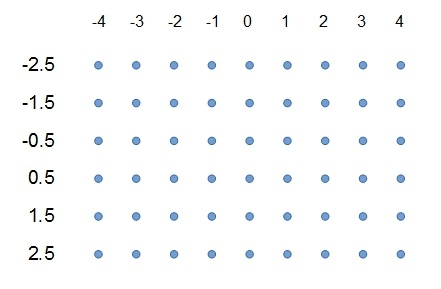
\includegraphics[scale=0.5]{images/object-points.jpg} 
\caption{Verteilung der Objektpunkt für ein Schachbrett.}
\label{fig:object-points}
\end{figure}


\subsection{Floating-point Ungenauigkeiten}

Ein Problem dass während des Projekts erst spät durch experimentieren gelöst werden konnte war, dass die berechnete und anschliessend dargestellte Projektion minimale Abweichungen aufweiste (siehe Abbildung \ref{floating-point-problem}). Das Problem war darauf zurückzuführen, dass die Algorithmen in OpenCV, die zur Lösung des PnP Problems verwendet wurden, scheinbar Probleme mit Gleitkommazahlen (engl. floating point) haben und dadurch das Resultat verfälschten.

Zur Lösung dieses Problems wurde ein möglichst einfacher Weg gewählt: Die Koordinaten der Objektpunkte wurden mit einem fix definierten Faktor von 100.0 hochskaliert. Dadurch wurden optisch erheblich bessere Resultate erzielt. Damit diese Methode anschliessend mit dem 3D-Rendering noch funktioniert, muss vor dem Rendering des 3D-Models die Model-View-Matrix entsprechend um den selben Skalierungsfaktor hochskaliert werden.

\begin{figure}[!ht]
\centering
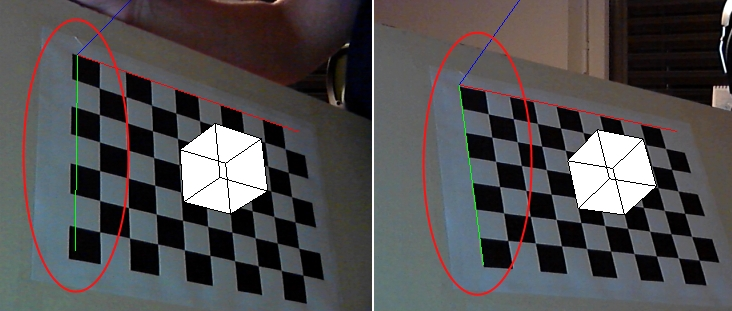
\includegraphics[scale=0.8]{images/floating-point-problem.jpg} 
\caption{Abweichung (links) vor der Optimierung (rechts).}
\label{fig:floating-point-problem}
\end{figure}


\section{Lagebestimmung einer Türe}

In diesem Kapitel wird die verwendete Methode zur Bestimmung der Lage einer Türe beschrieben.


\subsection{Grundidee}

\paragraph{}
Diese Grundidee zur Lagebestimmung einer Türe lässt sich anhand des Schachbrettmusters ableiten: Türe sowie Schachbrett sind beides rechteckige Objekte, dessen Eckpunkte ausserdem in der selben Ebene liegen. So wäre es physikalisch möglich, eine Türe mit dem Schachbrettmuster zu bemalen. 
Diese Idee wurde mit dieser Arbeit versucht virtuell zu entwickeln.
\\
\\
Als Input für die Lagebestimmung der Türe stehen genau deren vier Eckpunkte zur Verfügung. Diese werden von der Türerkennung generiert und bestehen aus einer X- und Y-Koordinaten, welche die Position eines Punktes im Ursprungsbild definieren. Ein erster Ansatz war, diese vier Bildpunkte weiteren vier vordefinierte Objektpunkten zuzuordnen und mittels eines PnP Algorithmus zu lösen. Die Objektpunkte wurden wie folgt definiert:

\begin{itemize}
\item \textbf{(0, 0)} oben links
\item \textbf{(1, 0)} oben rechts
\item \textbf{(1, 1)} unten rechts
\item \textbf{(0, 1)} unten links
\end{itemize}

Mit diesen Punkten wäre es theoretisch ebenfalls möglich, die Lage eines minimalen Schachbrettmusters (3x3) zu bestimmen. Das Problem im Falle einer Türe ist jedoch folgendes: Bei einem Schachbrettmuster sind die schwarzen bzw. weissen Flächen \textit{immer} Quadrate. Aus diesem Grund können die Objektpunkte ebenfalls als Quadrat definiert werden. Falls jedoch mit diesen Objektpunkten versucht wird die Lage eines nicht quadratischen Objekts, z.B. eine Türe, zu bestimmen, erhält man falsche Resultate. Da eine Türe auch kein standardisiertes Grössenverhältnis hat kann man keine vordefinierten Objektpunkte zur Lösung des Problems verwenden.

\subsection{Bestimmung des Grössenverhältnisses}

% TODO: evtl. noch Formeln aus Paper herleiten

\paragraph{}
In einer Arbeit von Zhengyou Zhang \cite{zhangrectification} wurde ein Verfahren entwickelt, mit welchem anhand genau vier Punkten eines Rechtecks dessen Grössenverhältnis berechnet werden kann. Hintergrund dieser Arbeit ist das automatische Erkennen von perspektivisch aufgenommenen Whiteboards mit anschliessender perspektivischen Entzerrung des Whiteboard-Inhalts.

Die Theorie funktioniert, weil bei den gegebenen Eckpunkten davon ausgegangen wird, dass diese sich in der gleichen Ebene befinden, was natürlich bei einem Whiteboard zutrifft. Aus diesem Grund kann auch für die Bestimmung des Grössenverthältnisses einer Türe dieses Verfahren herangezogen werden.

In Zhangs Dokument wird grundsätzlich von einer unkalibrierten Kamera ausgegangen und setzt bestimmte Kameraeigenschaften voraus, z.B. dass der Bildmittelpunkt genau in der Mitte ist, was bei einer Kamera nicht unbedingt der Fall sein muss. Zhang erwähnt auch, dass die Verzerrung der Kamera die Fehlerrate erhöhen kann. Da wir in unserem Modell von einer kalibrierten Kamera ausgehen, sind uns intrinsische Parameter und Verzerrung bekannt. Wir können deshalb vor der Anwendung des Algorithmus die Bildpunkte vorher entzerren.


\subsection{Messungen Grössenverhältnisse}

\paragraph{}
Zur Verifizierung der vorangehenden Arbeit von Zhang \cite{zhangrectification} wurden mit einer Spiegelreflexkamera hochauflösende Bilder einer Türe aufgenommen. Die Bilder wurden mit einem fixen Abstand zur Türe aufgenommen und ausgehend von der Türwand mit den Winkeln $10^\circ$, $30^\circ$, $50^\circ$, $70^\circ$ und $90^\circ$ aufgenommen. Anschliessend wurden die Koordinaten der vier Eckpunkte der Türe von Hand ausgelesen und mittels Algorithmus das Grössenverhältnis berechnet. Dieses wurde mit dem berechneten Verhältnis von \textbf{2.07} der aufgenommenen Türe mit den Massen \textbf{98.50cm x 204.00cm} verglichen.

\begin{center}
	\resizebox{\linewidth}{!}{%
    \begin{tabular}{ || l || l | l | l || l | l | l ||}
    \hline
    Winkel [$^\circ$] & Verhältnis (verzerrt) & Abweichung & Fehler & Verhältnis (entzerrt) & Abweichung & Fehler \\ \hline
    90 & 2.02 & 0.05 & 2.4 & 2.01 & 0.06 & 3.1 \\ \hline
    70 & 2.06 & 0.01 & 0.4 & 1.96 & 0.11 & 5.3 \\ \hline
    50 & 2.02 & 0.05 & 2.2 & 1.89 & 0.18 & 8.8 \\ \hline
    30 & 1.97 & 0.10 & 4.8 & 1.83 & 0.25 & 11.8 \\ \hline
    10 & 1.90 & 0.17 & 8.1 & 1.79 & 0.28 & 13.4 \\ \hline
    \end{tabular}
    }
\end{center}


\begin{figure}[!ht]
  \centering
  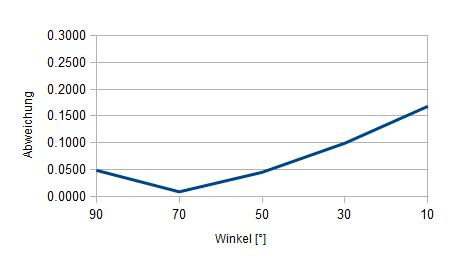
\includegraphics[width=0.75\linewidth]{images/ratio_v1_dist.jpg}
  \caption{Abweichung Grössenverhältnisse ohne Entzerrung, 1. Kalibration}
  \label{fig:ratio-v1-dist}
\end{figure}

\begin{figure}[!ht]
  \centering
  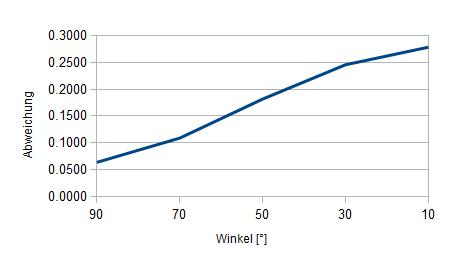
\includegraphics[width=0.75\linewidth]{images/ratio_v1_undist.jpg}
  \caption{Abweichung Grössenverhältnisse mit Entzerrung, 1. Kalibration}
  \label{fig:ratio-v1-undist}
\end{figure}


Die erste Durchführung der Messungen ergab ein unerwartetes Ergebnis. Der Verhältnis-Algorithmus wurde sowohl auf die verzerrten als auch die entzerrten Punkten angewendet. Überraschenderweise erhielten wir in der entzerrten Version schlechtere Resultate, was bei einer Spiegelreflexkamera verwunderlich ist, da diese eine sehr geringe Verzerrung haben sollte bzw. eine Entzerrung kameraseitig bereits durchführen sollte (siehe Abbildungen \ref{fig:ratio-v1-dist} und \ref{fig:ratio-v1-undist}).
\\
\\
Der Versuch wurde also ein zweites Mal gemacht. Diesmal wurde das Schachbrett zur Kalibration auf einer Spanpressblatte angebracht und möglichst flach aufgeklebt.


\begin{center}
	\resizebox{\linewidth}{!}{%
    \begin{tabular}{ || l || l | l | l || l | l | l ||}
    \hline
    Winkel [$^\circ$] & Verhältnis (verzerrt) & Abweichung & Fehler & Verhältnis (entzerrt) & Abweichung & Fehler \\ \hline
    90 & 2.01 & 0.06 & 2.7 & 2.01 & 0.06 & 2.8 \\ \hline
    70 & 2.03 & 0.04 & 2.0 & 2.03 & 0.03 & 1.8 \\ \hline
    50 & 2.03 & 0.04 & 1.8 & 2.04 & 0.03 & 1.4 \\ \hline
    30 & 2.06 & 0.01 & 0.3 & 2.06 & 0.01 & 0.3 \\ \hline
    10 & 2.07 & 0.00 & 0.0 & 2.06 & 0.01 & 0.7 \\ \hline
    \end{tabular}
    }
\end{center}

\begin{figure}[!ht]
  \centering
  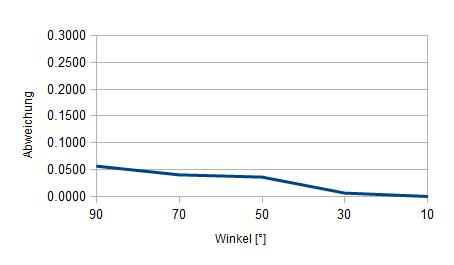
\includegraphics[width=0.75\linewidth]{images/ratio_v2_dist.jpg}
  \caption{Abweichung Grössenverhältnisse ohne Entzerrung, 2. Kalibration}
  \label{fig:ratio-v2-dist}
\end{figure}

\begin{figure}[!ht]
  \centering
  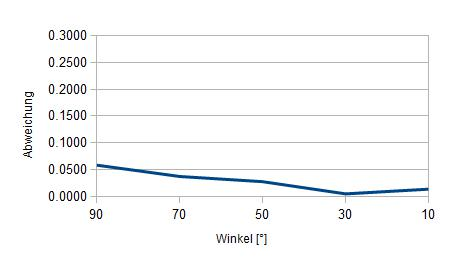
\includegraphics[width=0.75\linewidth]{images/ratio_v2_undist.jpg}
  \caption{Abweichung Grössenverhältnisse mit Entzerrung, 2. Kalibration}
  \label{fig:ratio-v2-undist}
\end{figure}


Die zweiten Resultate entsprachen nun den erwarteten Werten. Auf den Abbildungen \ref{fig:ratio-v2-dist} und \ref{fig:ratio-v2-undist}) ist gut zu erkennen, dass sowohl die verzerrte als auch die entzerrte Version ähnliche Resultate zurückliefert, was von einer Spiegelreflexkamera erwartet werden sollte. Zudem haben wir einen maximalen Fehlerwert von 2.8 Prozent messen können, was ein guter Wert ist. Der Versuch hat zudem gezeit, dass eine schlecht kalibrierte Kamera erhebliche Verfälschungen des Resultats zur Folge haben kann. 


\subsection{Umsetzung}

\paragraph{}
Da nun, wie in den vorherigen Abschnitten beschrieben, das Grössenverhältnis der Türe berechnet werden kann, können wir den ursprünglichen Ansatz mit dem zuordnen von Objektpunkten weiterverfolgen. Die Objektpunkte werden nun jedoch nicht vordefiniert, sondern bei der Lagebestimmung automatisch anhand des Grössenverhältnisses generiert. Dabei wird als \textbf{Breite 1} angenommen und als \textbf{Höhe das Verhältnis r}. Die generierten Punkte werden wie folgt generiert:

\begin{itemize}
\item \textbf{(0, 0)} unten links
\item \textbf{(0, r)} oben links
\item \textbf{(1, r)} oben rechts
\item \textbf{(0, 1)} unten rechts
\end{itemize}

Diese Punkte können nun zusammen mit den erkannten Eckpunkten der Türe an einen PnP Algorithmus übergeben werden, welcher die Position und Rotation berechnet.


\newpage


\chapter{Projektion in OpenGL}

Durch die Objekterkennung und anschliessender Bestimmung dessen Lage wurde ein wichtiger Teil zur Fertigstellung einer Augmented Reality Szene bereits erreicht. Im letzten Schritt geht es nun darum, die Resultate aus den vorhergehenden Schritten zu verwenden und schlussendlich ein 3D-Objekt mit korrekter Perspektive in die Szene zu rendern.


\section{Livebild mittels Texturemapping}

Da wir für eine Augmented Reality Szene immer auch die Realität als Hintergrund betrachten wollen, müssen wir das Livebild der Kamera ebenfalls in die dreidimensionale Szene integrieren. Dies erreichen wir, indem wir für jedes Einzelbild der Kamera ein \textit{Texture Mapping} durchführen.
Der Ablauf des Texture Mappings kann vereinfacht mit folgenden Schritten in OpenGL aufgezeigt werden:

\begin{enumerate}
\item Das Bild wird in eine Textur konvertiert und auf die Grafikkarte hochgeladen.
\item Zeichne ein planares, rechteckiges Objekt in die Szene.
\item Entsprechend der definierten Textur-Koordinaten zeichnet die Grafikkarte die Oberfläche des Objekts mit der Textur.
\end{enumerate}

Ausserdem wird für diesen Schritt eine orthogonale Projektion durchgeführt, damit das gerenderte Hintergrundbild die gleichen Dimensionen hat, egal ob es sich vorne oder hinten in der Szene befindet. Wir können dadurch das Hintergrundbild weit nach hinten schieben, so dass es keine Kollision mit den später zu rendernden Objekten gibt.


\section{Transformation der extrinsischen Matrix}

Durch die pose estimation konnte bereits die extrinsische Matrix bestimmt werden. Damit ein in OpenGL gerendertes Objekt an der selben Position mit der selben Rotation wie das real erkannte Objekt erscheint, muss die extrinsische Matrix an OpenGL übergeben werden.


\begin{figure}[!ht]
\centering
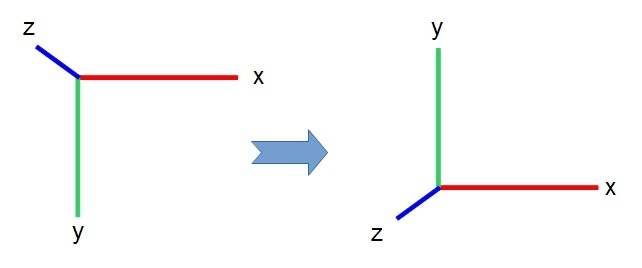
\includegraphics[scale=0.5]{images/opencv-to-opengl.jpg} 
\caption{Transformierung des Koordinatensystem von OpenCV (links) nach OpenGL (rechts).}
\label{fig:opencv-to-opengl}
\end{figure}


Die Matrix aus OpenCV kann jedoch nicht direkt an OpenGL übergeben werden, da die beiden unterschiedliche Koordinatensysteme verwenden. Die Abbildung \ref{fig:opencv-to-opengl} stellt diese Gegebenheit grafisch dar. Die Konvertierung kann mit einer einfachen Matrixmultiplikation erreicht werden, indem die Y- und Z-Achsen invertiert werden:

\begin{equation}
M_{OpenGL}
=
\begin{bmatrix}
1 & 0 & 0 & 0 \\
0 & -1 & 0 & 0 \\
0 & 0 & -1 & 0 \\
0 & 0 & 0 & 1
\end{bmatrix} 
[R | t]
\end{equation}

 
\section{Perspektivische Projektion}

Damit ein virtuelles Objekt sich in die reale Szene einfügen kann, muss die korrekte perspektivische Projektion gesetzt werden, nämlich dieselbe, welche auch die Kamera hatte, die das reale Bild aufgenommen hat. Die dazu benötigte Projektionsmatrix kann anhand der \textit{intrinsischen Parameter} abgeleitet werden. Ein Vergleich einer inkorrekten Projektionsmatrix mit einer korrekten ist in Abbildung \ref{fig:opengl-perspektive} zu sehen.


\begin{figure}[!ht]
\centering
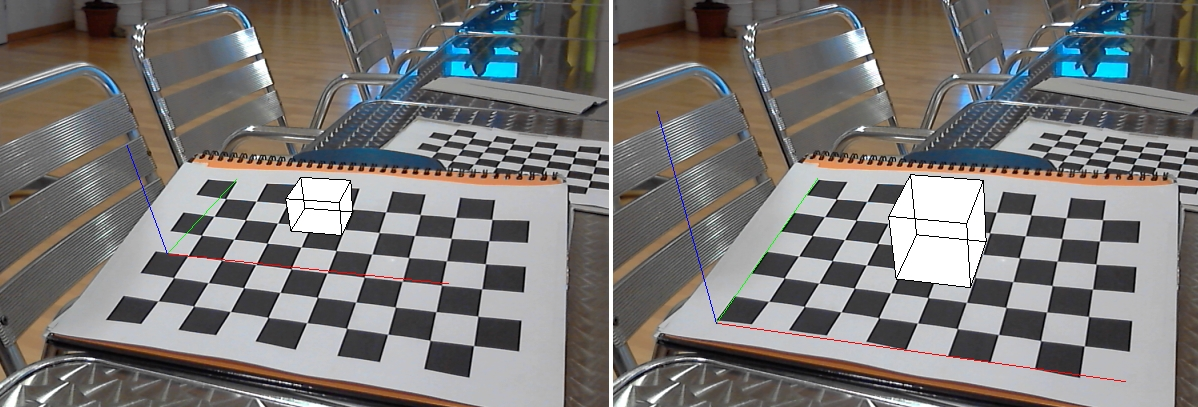
\includegraphics[scale=0.5]{images/opengl-perspective.jpg} 
\caption{Eine inkorrekt gesetzt perspektivische Projektion oder falsche intrinsische Parameter können das projizierte Objekt stark verfälschen.}
\label{fig:opengl-perspektive}
\end{figure}


K. Simek \cite{simek} erklärt die notwendigen Schritte, wie die perspektivische Projektion anhand der Kameramatrix gesetzt werden kann. Er teilt dazu die Projektionsmatrix dazu in die Teile Perspektive und NDC (Normalized Device Coordinates) auf (Gleichung \ref{eq:projektion}).

\begin{equation}
Proj = NDC * Persp
\label{eq:projektion}
\end{equation}

Der NDC kann in OpenGL mit einer orthogonalen Projektion umgesetzt werden. Die Perspektivenmatrix muss mit den kameraspezifischen intrinsischen Parametern ergänzt werden. $\alpha$ und $\beta$ entsprechen dabei der horizontalen und vertikalen Brennweiten der Kamera, $x_0$ und $y_0$ der Abweichung der optischen Bildmitte zum Bildzentrum. Die resultierende Projektionsmatrix kann später direkt in OpenGL angewandt werden.

\begin{equation}
Persp
=
\begin{bmatrix}
\alpha & 0 & -x_0 & 0 \\
0 & \beta & -y_0 & 0 \\
0 & 0 & near + far & near * far \\
0 & 0 & -1 & 0
\end{bmatrix} 
\end{equation}


\section{Positionierung der 3D Objekte}

Wie bereits in Kapitel \ref{sec:projektion-door} beschrieben, wurden die Objektpunkte einer Türe so definiert, dass die untere linke Ecke als Ursprungspunkt (0, 0) dient. Da ein Ziel dieser Arbeit ist, ein Vordach über die Türe zu prjizieren, muss eine entsprechende Translation vorgenommen werden.

Da keine Kenntnisse über die realen Einheiten (siehe Kapitel \ref{sec:definition-objektpunkte}) bekannt sind, müssen wir die Translation entsprechend der Einheit der definierten Objektpunkte durchführen. Da die Breite der Türe als Einheitsgrösse 1 definiert wurde und die Höhe dem Verhältnis Höhe zu Breite entspricht, können wir die Model-View-Matrix um die halbe Breite (0.5) und die Höhe (r = Verhältnis Höhe zu Breite) verschieben (Abbildung \ref{fig:opengl-translation}).

\begin{equation}
M_{translation}
=
\begin{bmatrix}
1 & 0 & 0 & w/2 \\
0 & 1 & 0 & h \\
0 & 0 & 1 & 0 \\
0 & 0 & 0 & 1
\end{bmatrix} 
\end{equation}


\begin{figure}[!ht]
\centering
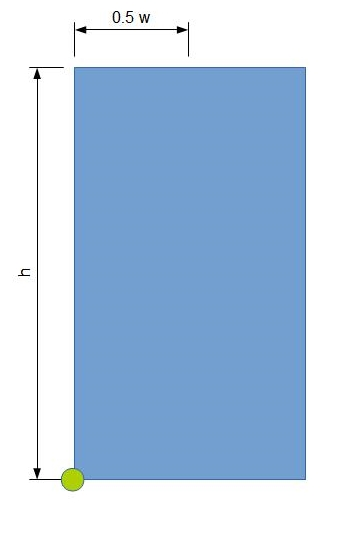
\includegraphics[scale=0.75]{images/opengl-translation.jpg} 
\caption{Schematische Darstellung der Translation von der unteren linken Ecke der Türe zur Oberkante.}
\label{fig:opencv-perspektive}
\end{figure}


\section{Konvertierung nach Core Profile}

Nach einer ersten funktionierenden Version der Schachbretterkennung inklusive Projektion und 3D-Rendering haben wir Zeit in die Konvertierung nach Core Profile OpenGL investiert. Diesen Schritt haben wir gewählt, weil die in dieser Version zur Verfügung stehenden Routinen ebenfalls auf den mobilen Versionen von OpenGL (OpenGL ES) zu finden und eine zukünftige Portierung dadurch erheblich vereinfacht wird. Core Profile wird aktuell auch als moderne Art der OpenGL-Entwicklung betrachtet und bietet eine vereinfachte API und bessere Performance.



\newpage

\chapter{Resultat}

\section{Ardoor Library}

\section{Settings App}

\section{Calibration App}

\section{Chessboard App}

\section{Door App}


\newpage

\chapter{Fazit}

Insgesamt sind wir mit unserer Arbeit zufrieden und konnten unser Hauptziel zum gr�ssten Teil erreichen. Wir k�nnen T�ren in einem Livebild erkennen und deren Position und Rotation bestimmen. Die Arbeit war f�r uns eine grosse Herausforderung, da wir beide vorher nur wenig bis gar keine Erfahrung auf den unterschiedlichen Gebieten dieses Projekts hatten.

Probleme gibt es noch bei Erkennung von seitlich betrachteten T�ren. Hier funktioniert die Erkennung noch nicht zuverl�ssig. Wir haben zu sp�t realisiert, dass wir f�r die perspektivische Erkennung zus�tzliche Verfahren h�tten evaluieren sollen, z.B. die Klassifizierung von Linien anhand der Tendenz zu einem Fluchtpunkt.

% TODO evtl. mit Resultat verschmelze?


Da wir haben mit unserer Arbeit in erster Linie eine Grundlage geschaffen haben, gibt es definitiv zus�tzliches Optimiers- und Erweiterungspotential.

Sinnvoll w�re eine Optimierung der Performance der Algorithmen, besonders im Bereich der T�rerkennung. Hier haben wir prim�r auf die Funktionalit�t konzentriert. 

Ein wichtiger n�chster Schritt wird sein, die Anwendung auf mobile Plattformen zu portieren. Durch die immer h�ufigere Verbreitung von Smartphones und die M�glichkeit, Informationen an Ort und Stelle abzurufen, oder im Falle von Augmented Reality direkt einzublenden, sind solche Ger�te eine gew�nschte Zielgruppe. 

Ein Ausblick in die Zukunft der Augmented Reality sieht ebenfalls vielversprechend aus. Grosses Aufsehen sorgte diesbez�glich vorallem Google, die mit ihrem Produkt Glass versuchen Augmented Reality Massentauglich zu machen. Besonders in Alltagssituation k�nnte Augmented Reality eine grosse Rolle einnehmen, beispielsweise durch Navigationshilfen in Autos, die n�tzliche Informationen direkt auf die Frontscheibe projizieren.

Aber auch f�r unseren Spezialfall der Augmented Reality kann man sich verschiedene Anwendungszwecke vorstellen. Das Einkaufen k�nnte interaktiver werden, indem Dinge wie M�bel als Modelle auf das eigene Smartphone geladen werden. Mittels einer Augmented Reality App k�nnen diese direkt in der aktuellen Umgebung von allen Seiten betrachtet werden. Dies k�nne zudem mit aufkommenden Techniken wie NFC (Near Field Communication) erweitert werden: Man stelle sich eine Einkaufstour durch ein M�belhaus seiner Wahl vor. Mittels NFC k�nnen 3D-Modelle von M�beln direkt auf das Smartphone geladen werden. Sp�ter kann man die ausgesuchten Gegenst�nde in der eigenen Wohnung virtuell platzieren und dadurch eine bessere Kaufentscheidung f�llen.


\newpage

\begin{thebibliography}{5}

\bibitem {learningopencv}
Bradski, Gary / Kaehler Adrian:
Learning OpenCV: Computer Vision with the OpenCV Library.
Sebastopol: O'Reilly Media, Inc.

\bibitem {zhang}
Zhang, Zhengyou (1998): A Flexible New Technique for Camera Calibration. 
Redmond: Microsoft Research.

\bibitem {escalera}
de la Escalera, Arturo / María Armingol, Jose: Automatic Chessboard Detection for Intrinsic and Extrinsic Camera Parameter Calibration. 
Madrid: Universidad Carlos III de Madrid.

\bibitem {kiryati}
N. Kiryati, Y. Eldar, A.M. Bruckstein:
A probabilistic Hough transform, Pattern Recognition 
Volume 24, Issue 4, 1991, Pages 303-316, ISSN 0031-3203, DOI: 10.1016/0031-3203(91)90073-E. 

\bibitem {nieto}
Nieto, Marcos (2011): Line segment detection using weighted mean shift procedures on a 2D slice sampling strategy
London: Springer

\bibitem {bresenham}
Bresenham, Jack (1965): Algorithm for computer control of a digital plotter. 
USA: IBM

\bibitem {zhangrectification}
Zhang, Zhengyou (2002): Single-View Geometry of A Rectangle With Application to Whiteboard Image Rectification.
Redmond: Microsoft Research.

\bibitem {simek}
Simek, Kyle: Calibrated Cameras in OpenGL without glFrustum. Stand 03. Juni 2013. $http://ksimek.github.io/2013/06/03/calibrated_cameras_in_opengl$  (aufgerufen am 16. Januar 2013).


\end{thebibliography}

\newpage
\chapter{Ehrlichkeitserklärung}
Hiermit bestätigen die Autoren, diese Arbeit ohne fremde Hilfe und unter Einhaltung der gebotenen Regeln erstellt zu haben.
\\
\\
\\
\textbf{Mato Ilic}
\\
\\
\\
\rule{0.85\textwidth}{0.4pt} \\
Ort, Datum \hspace * {5cm} Unterschrift
\\
\\
\\
\textbf{David Kron}
\\
\\
\\
\rule{0.85\textwidth}{0.4pt} \\
Ort, Datum \hspace * {5cm} Unterschrift

\newpage
\chapter{Anhang}

\section{Schachbrett für Kalibrierung}

\newpage


\includegraphics[width=\textwidth]{images/chessboard}

\chapter{Messungen Door Ratio Algorithmus}
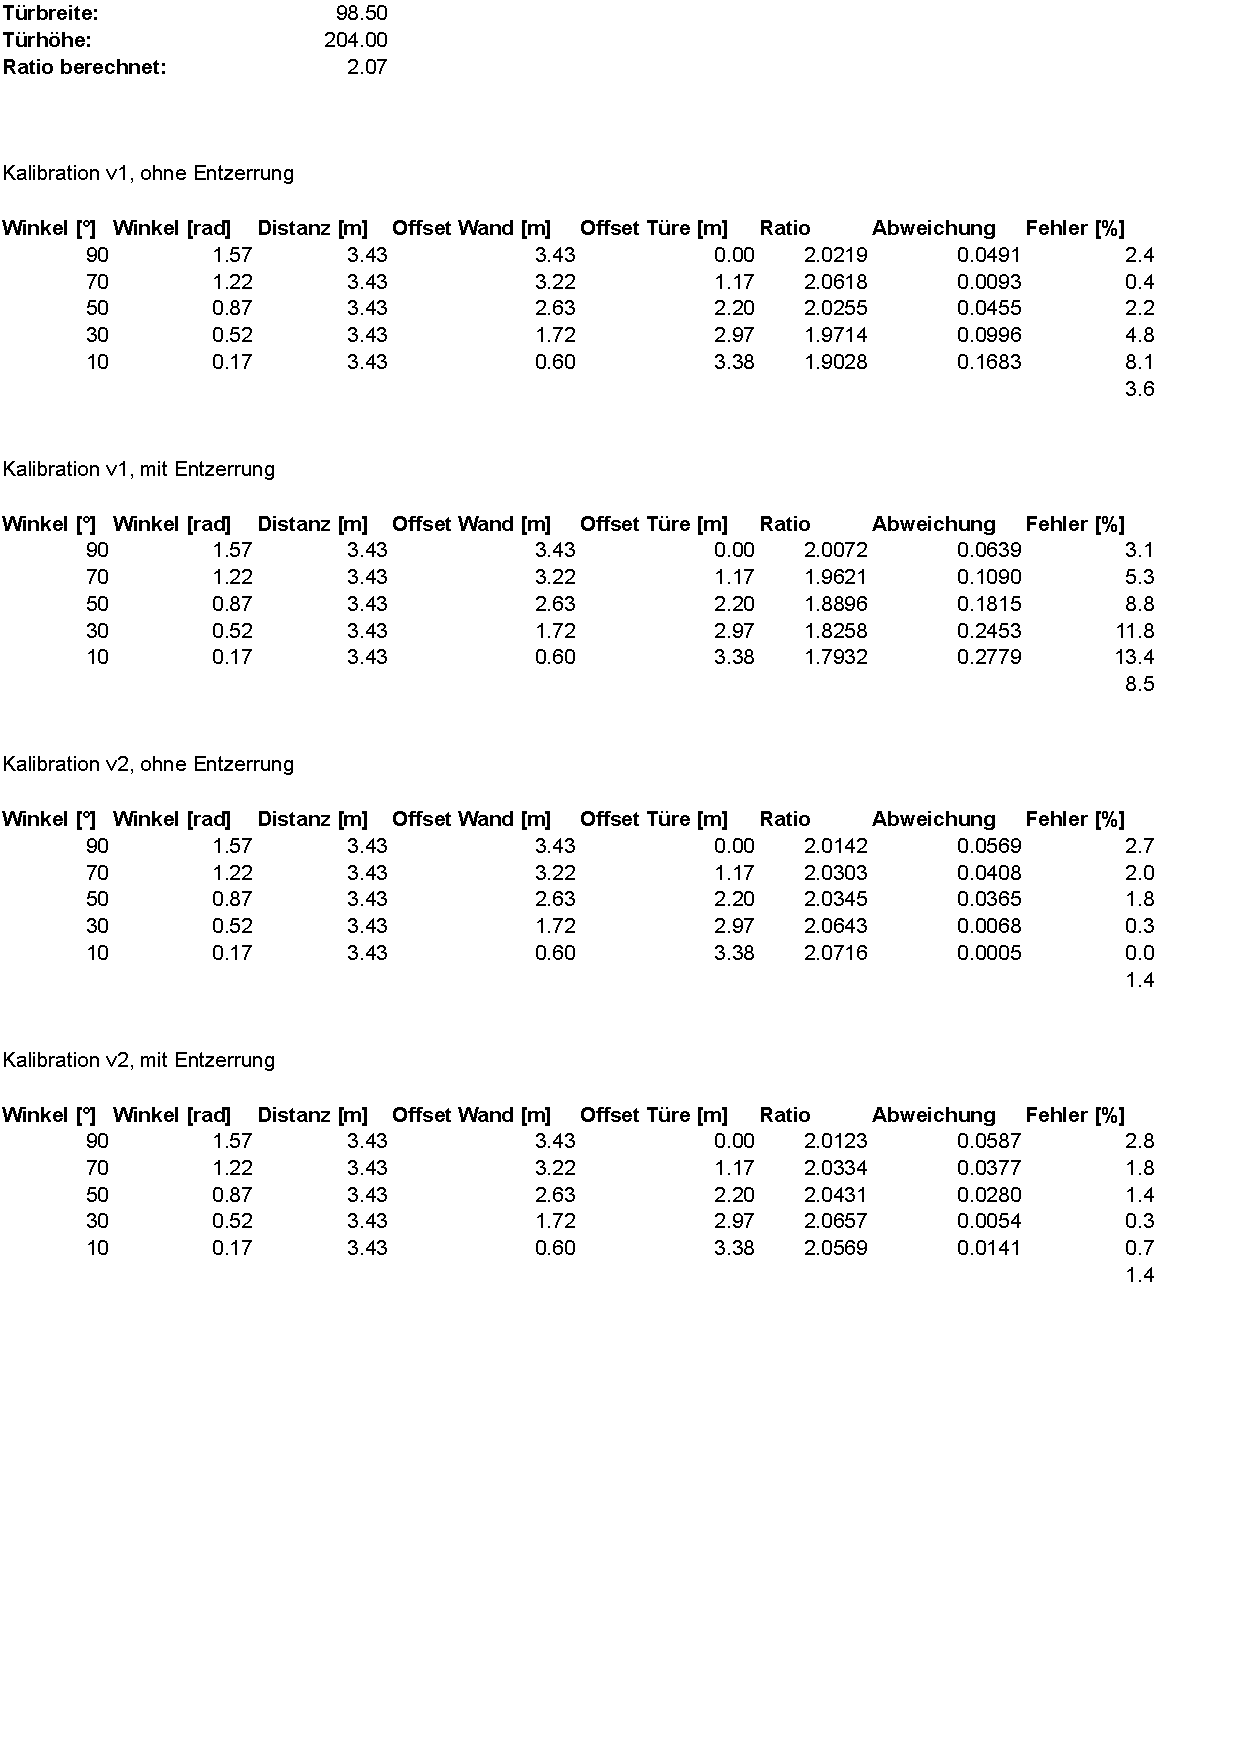
\includegraphics[width=\textwidth]{images/messurements}

\end{document}
